\documentclass[]{article}
\usepackage{lmodern}
\usepackage{amssymb,amsmath}
\usepackage{ifxetex,ifluatex}
\usepackage{fixltx2e} % provides \textsubscript
\ifnum 0\ifxetex 1\fi\ifluatex 1\fi=0 % if pdftex
  \usepackage[T1]{fontenc}
  \usepackage[utf8]{inputenc}
\else % if luatex or xelatex
  \ifxetex
    \usepackage{mathspec}
  \else
    \usepackage{fontspec}
  \fi
  \defaultfontfeatures{Ligatures=TeX,Scale=MatchLowercase}
\fi
% use upquote if available, for straight quotes in verbatim environments
\IfFileExists{upquote.sty}{\usepackage{upquote}}{}
% use microtype if available
\IfFileExists{microtype.sty}{%
\usepackage{microtype}
\UseMicrotypeSet[protrusion]{basicmath} % disable protrusion for tt fonts
}{}
\usepackage[margin=1in]{geometry}
\usepackage{hyperref}
\hypersetup{unicode=true,
            pdftitle={Buzz vs.~Bite},
            pdfborder={0 0 0},
            breaklinks=true}
\urlstyle{same}  % don't use monospace font for urls
\usepackage{color}
\usepackage{fancyvrb}
\newcommand{\VerbBar}{|}
\newcommand{\VERB}{\Verb[commandchars=\\\{\}]}
\DefineVerbatimEnvironment{Highlighting}{Verbatim}{commandchars=\\\{\}}
% Add ',fontsize=\small' for more characters per line
\usepackage{framed}
\definecolor{shadecolor}{RGB}{248,248,248}
\newenvironment{Shaded}{\begin{snugshade}}{\end{snugshade}}
\newcommand{\KeywordTok}[1]{\textcolor[rgb]{0.13,0.29,0.53}{\textbf{#1}}}
\newcommand{\DataTypeTok}[1]{\textcolor[rgb]{0.13,0.29,0.53}{#1}}
\newcommand{\DecValTok}[1]{\textcolor[rgb]{0.00,0.00,0.81}{#1}}
\newcommand{\BaseNTok}[1]{\textcolor[rgb]{0.00,0.00,0.81}{#1}}
\newcommand{\FloatTok}[1]{\textcolor[rgb]{0.00,0.00,0.81}{#1}}
\newcommand{\ConstantTok}[1]{\textcolor[rgb]{0.00,0.00,0.00}{#1}}
\newcommand{\CharTok}[1]{\textcolor[rgb]{0.31,0.60,0.02}{#1}}
\newcommand{\SpecialCharTok}[1]{\textcolor[rgb]{0.00,0.00,0.00}{#1}}
\newcommand{\StringTok}[1]{\textcolor[rgb]{0.31,0.60,0.02}{#1}}
\newcommand{\VerbatimStringTok}[1]{\textcolor[rgb]{0.31,0.60,0.02}{#1}}
\newcommand{\SpecialStringTok}[1]{\textcolor[rgb]{0.31,0.60,0.02}{#1}}
\newcommand{\ImportTok}[1]{#1}
\newcommand{\CommentTok}[1]{\textcolor[rgb]{0.56,0.35,0.01}{\textit{#1}}}
\newcommand{\DocumentationTok}[1]{\textcolor[rgb]{0.56,0.35,0.01}{\textbf{\textit{#1}}}}
\newcommand{\AnnotationTok}[1]{\textcolor[rgb]{0.56,0.35,0.01}{\textbf{\textit{#1}}}}
\newcommand{\CommentVarTok}[1]{\textcolor[rgb]{0.56,0.35,0.01}{\textbf{\textit{#1}}}}
\newcommand{\OtherTok}[1]{\textcolor[rgb]{0.56,0.35,0.01}{#1}}
\newcommand{\FunctionTok}[1]{\textcolor[rgb]{0.00,0.00,0.00}{#1}}
\newcommand{\VariableTok}[1]{\textcolor[rgb]{0.00,0.00,0.00}{#1}}
\newcommand{\ControlFlowTok}[1]{\textcolor[rgb]{0.13,0.29,0.53}{\textbf{#1}}}
\newcommand{\OperatorTok}[1]{\textcolor[rgb]{0.81,0.36,0.00}{\textbf{#1}}}
\newcommand{\BuiltInTok}[1]{#1}
\newcommand{\ExtensionTok}[1]{#1}
\newcommand{\PreprocessorTok}[1]{\textcolor[rgb]{0.56,0.35,0.01}{\textit{#1}}}
\newcommand{\AttributeTok}[1]{\textcolor[rgb]{0.77,0.63,0.00}{#1}}
\newcommand{\RegionMarkerTok}[1]{#1}
\newcommand{\InformationTok}[1]{\textcolor[rgb]{0.56,0.35,0.01}{\textbf{\textit{#1}}}}
\newcommand{\WarningTok}[1]{\textcolor[rgb]{0.56,0.35,0.01}{\textbf{\textit{#1}}}}
\newcommand{\AlertTok}[1]{\textcolor[rgb]{0.94,0.16,0.16}{#1}}
\newcommand{\ErrorTok}[1]{\textcolor[rgb]{0.64,0.00,0.00}{\textbf{#1}}}
\newcommand{\NormalTok}[1]{#1}
\usepackage{longtable,booktabs}
\usepackage{graphicx,grffile}
\makeatletter
\def\maxwidth{\ifdim\Gin@nat@width>\linewidth\linewidth\else\Gin@nat@width\fi}
\def\maxheight{\ifdim\Gin@nat@height>\textheight\textheight\else\Gin@nat@height\fi}
\makeatother
% Scale images if necessary, so that they will not overflow the page
% margins by default, and it is still possible to overwrite the defaults
% using explicit options in \includegraphics[width, height, ...]{}
\setkeys{Gin}{width=\maxwidth,height=\maxheight,keepaspectratio}
\IfFileExists{parskip.sty}{%
\usepackage{parskip}
}{% else
\setlength{\parindent}{0pt}
\setlength{\parskip}{6pt plus 2pt minus 1pt}
}
\setlength{\emergencystretch}{3em}  % prevent overfull lines
\providecommand{\tightlist}{%
  \setlength{\itemsep}{0pt}\setlength{\parskip}{0pt}}
\setcounter{secnumdepth}{0}
% Redefines (sub)paragraphs to behave more like sections
\ifx\paragraph\undefined\else
\let\oldparagraph\paragraph
\renewcommand{\paragraph}[1]{\oldparagraph{#1}\mbox{}}
\fi
\ifx\subparagraph\undefined\else
\let\oldsubparagraph\subparagraph
\renewcommand{\subparagraph}[1]{\oldsubparagraph{#1}\mbox{}}
\fi

%%% Use protect on footnotes to avoid problems with footnotes in titles
\let\rmarkdownfootnote\footnote%
\def\footnote{\protect\rmarkdownfootnote}

%%% Change title format to be more compact
\usepackage{titling}

% Create subtitle command for use in maketitle
\newcommand{\subtitle}[1]{
  \posttitle{
    \begin{center}\large#1\end{center}
    }
}

\setlength{\droptitle}{-2em}

  \title{Buzz vs.~Bite}
    \pretitle{\vspace{\droptitle}\centering\huge}
  \posttitle{\par}
  \subtitle{An Analysis of Alcohol Content and Bitterness in American Craft Beers}
  \author{}
    \preauthor{}\postauthor{}
      \predate{\centering\large\emph}
  \postdate{\par}
    \date{June 26, 2018}

\usepackage{amsmath}
\usepackage{mathtools}
\usepackage{float}
\usepackage{xcolor,pifont}
\newcommand{\cmark}{\Large\textcolor{green}{\ding{52}}}
\newcommand{\xmark}{\Large\textcolor{red}{\ding{55}}}
\usepackage{blindtext}
\usepackage[utf8]{inputenc}

\begin{document}
\maketitle

\subsection{Introduction}\label{introduction}

It goes without saying that entering the craft beer market, in pretty
much any state, is a monstrous task. The explosion of micro-breweries
has spread expeditiously in nearly every rapidly-growing urban
environment. Luckily for you, the explosion is not in isolation. Demand
has never been higher for unique and complex alcoholic libations. Where
once the thought process was ``the simpler the better,'' newer
generations are constantly on the hunt for a drinking experience that
fits their lifestyle and temperament. Although the market may seem
saturated in many areas, it is, in reality, a rich field filled with
almost never-ending demand ready to be tapped by the right combination
of ingenuity, experimentation and a knowledge of what sells.

\subsection{Purpose of this study}\label{purpose-of-this-study}

Purpose of this study * To organize and analyze a list of 2410 craft
beers from the United States and a list of 558 breweries. * To help you
identify trends within this data to help narrow your focus for
production. Manufacturing a beer that will outsell your competitors is
more than just a quality product, it's knowing what quality is proven to
sell. * To provide you with a functional list of each beer's alcohol
content, bitterness level, style and other information to help you
decide which direction to take your production facilities and supply
chain.

\subsection{Loading required
libraries}\label{loading-required-libraries}

The following code loads useful libraries that aren't included in base
R. The of these libraries come from the ``tidyverse'' including dplyr
for manipulating dataframes, tidyr for making data tidy, knitr for
creating reproducible documents ggplot2 for plots, maps for help with
geographic plots, RColorBrewer for improved map graphics, summarytools
for summarizing data, magrittr for better code, and gridExtra to assist
with plots

\begin{verbatim}
## Loading required package: dplyr
\end{verbatim}

\begin{verbatim}
## 
## Attaching package: 'dplyr'
\end{verbatim}

\begin{verbatim}
## The following objects are masked from 'package:stats':
## 
##     filter, lag
\end{verbatim}

\begin{verbatim}
## The following objects are masked from 'package:base':
## 
##     intersect, setdiff, setequal, union
\end{verbatim}

\begin{verbatim}
## Loading required package: tidyr
\end{verbatim}

\begin{verbatim}
## Loading required package: knitr
\end{verbatim}

\begin{verbatim}
## Loading required package: ggplot2
\end{verbatim}

\begin{verbatim}
## Loading required package: maps
\end{verbatim}

\begin{verbatim}
## Loading required package: RColorBrewer
\end{verbatim}

\begin{verbatim}
## Loading required package: summarytools
\end{verbatim}

\begin{verbatim}
## Loading required package: magrittr
\end{verbatim}

\begin{verbatim}
## 
## Attaching package: 'magrittr'
\end{verbatim}

\begin{verbatim}
## The following object is masked from 'package:tidyr':
## 
##     extract
\end{verbatim}

\begin{verbatim}
## Loading required package: gridExtra
\end{verbatim}

\begin{verbatim}
## 
## Attaching package: 'gridExtra'
\end{verbatim}

\begin{verbatim}
## The following object is masked from 'package:dplyr':
## 
##     combine
\end{verbatim}

\subsection{Breweries Data}\label{breweries-data}

\subsubsection{Import Breweries}\label{import-breweries}

In this section we load and begin cleaning the data in order to aid our
exploratory analysis. Column names are set to lowercase for ease of
reading and we begin to summarize the data.

\begin{Shaded}
\begin{Highlighting}[]
\CommentTok{#import breweries data}
\NormalTok{breweries_data <-}\StringTok{ }\KeywordTok{read.csv}\NormalTok{(}\StringTok{"../data/Breweries.csv"}\NormalTok{, }\DataTypeTok{header=}\OtherTok{TRUE}\NormalTok{)}


\KeywordTok{colnames}\NormalTok{(breweries_data) }\OperatorTok\StringTok{ }\NormalTok{tolower }\CommentTok{#lower case colnames}

\NormalTok{breweries_data }\OperatorTok\StringTok{ }\KeywordTok{rename}\NormalTok{(}\DataTypeTok{brewery_id =}\NormalTok{ brew_id) }\CommentTok{#rename}
\end{Highlighting}
\end{Shaded}

\subsubsection{Inspect Raw Breweries
Dataset}\label{inspect-raw-breweries-dataset}

\begin{Shaded}
\begin{Highlighting}[]
\CommentTok{# count breweries by state}
\NormalTok{brewery_summary_raw <-}\StringTok{ }\KeywordTok{select}\NormalTok{(breweries_data, state, brewery_id) }\OperatorTok\StringTok{ }\CommentTok{#select columns}
\StringTok{                   }\NormalTok{dplyr}\OperatorTok{::}\KeywordTok{group_by}\NormalTok{(state) }\OperatorTok\StringTok{ }\CommentTok{#group by}
\StringTok{                   }\NormalTok{dplyr}\OperatorTok{::}\KeywordTok{summarize_all}\NormalTok{(}\KeywordTok{funs}\NormalTok{(}\KeywordTok{n_distinct}\NormalTok{(.))) }\OperatorTok
\StringTok{                   }\KeywordTok{arrange}\NormalTok{(}\KeywordTok{desc}\NormalTok{(brewery_id))}



\CommentTok{# print top 5 states with the most breweries}
\KeywordTok{kable}\NormalTok{(}\KeywordTok{head}\NormalTok{(brewery_summary_raw, }\DecValTok{5}\NormalTok{), }\DataTypeTok{digits =} \DecValTok{0}\NormalTok{)}
\end{Highlighting}
\end{Shaded}

\begin{longtable}[]{@{}lr@{}}
\toprule
state & brewery\_id\tabularnewline
\midrule
\endhead
CO & 47\tabularnewline
CA & 39\tabularnewline
MI & 32\tabularnewline
OR & 29\tabularnewline
TX & 28\tabularnewline
\bottomrule
\end{longtable}

\begin{Shaded}
\begin{Highlighting}[]
\CommentTok{# print bottom 5 states with the most breweries}
\KeywordTok{kable}\NormalTok{(}\KeywordTok{tail}\NormalTok{(brewery_summary_raw, }\DecValTok{5}\NormalTok{), }\DataTypeTok{digits =} \DecValTok{0}\NormalTok{)}
\end{Highlighting}
\end{Shaded}

\begin{longtable}[]{@{}lr@{}}
\toprule
state & brewery\_id\tabularnewline
\midrule
\endhead
NV & 2\tabularnewline
DC & 1\tabularnewline
ND & 1\tabularnewline
SD & 1\tabularnewline
WV & 1\tabularnewline
\bottomrule
\end{longtable}

\begin{Shaded}
\begin{Highlighting}[]
\KeywordTok{ggplot}\NormalTok{(brewery_summary_raw) }\OperatorTok{+}
\StringTok{      }\KeywordTok{geom_bar}\NormalTok{(}\KeywordTok{aes}\NormalTok{(}\DataTypeTok{x =} \KeywordTok{reorder}\NormalTok{(state, }\OperatorTok{-}\NormalTok{brewery_id, }\DataTypeTok{FUN=}\NormalTok{max),}
                   \DataTypeTok{y =}\NormalTok{ brewery_id), }
               \DataTypeTok{stat =}\StringTok{"identity"}\NormalTok{,}
               \DataTypeTok{fill =}\NormalTok{ misc_cool) }\OperatorTok{+}
\StringTok{      }\KeywordTok{guides}\NormalTok{(}\DataTypeTok{fill=}\KeywordTok{guide_legend}\NormalTok{(}\DataTypeTok{title=} \OtherTok{NULL}\NormalTok{)) }\OperatorTok{+}
\StringTok{      }\KeywordTok{xlab}\NormalTok{(}\OtherTok{NULL}\NormalTok{) }\OperatorTok{+}
\StringTok{      }\KeywordTok{ylab}\NormalTok{(}\StringTok{"Number of Beer Styles"}\NormalTok{) }\OperatorTok{+}
\StringTok{      }\KeywordTok{scale_y_continuous}\NormalTok{(}\DataTypeTok{breaks =} \KeywordTok{c}\NormalTok{(}\DecValTok{0}\NormalTok{, }\DecValTok{10}\NormalTok{, }\DecValTok{20}\NormalTok{, }\DecValTok{30}\NormalTok{, }\DecValTok{40}\NormalTok{, }\DecValTok{50}\NormalTok{), }
                         \DataTypeTok{limits =} \KeywordTok{c}\NormalTok{(}\DecValTok{0}\NormalTok{, }\DecValTok{50}\NormalTok{), }
                         \DataTypeTok{minor_breaks =} \KeywordTok{c}\NormalTok{(}\DecValTok{5}\NormalTok{, }\DecValTok{15}\NormalTok{, }\DecValTok{25}\NormalTok{, }\DecValTok{35}\NormalTok{ ,}\DecValTok{45}\NormalTok{)) }\OperatorTok{+}
\StringTok{      }\KeywordTok{ggtitle}\NormalTok{(}\StringTok{"Count of Beer Styles by State"}\NormalTok{) }\OperatorTok{+}
\StringTok{      }\KeywordTok{theme}\NormalTok{(}\DataTypeTok{plot.title =} \KeywordTok{element_text}\NormalTok{(}\DataTypeTok{hjust =} \FloatTok{0.5}\NormalTok{)) }\OperatorTok{+}\StringTok{ }\CommentTok{# center plot title}
\StringTok{      }\KeywordTok{theme}\NormalTok{(}\DataTypeTok{text =} \KeywordTok{element_text}\NormalTok{(}\DataTypeTok{size=}\DecValTok{10}\NormalTok{),}
            \DataTypeTok{axis.text.x =} \KeywordTok{element_text}\NormalTok{(}\DataTypeTok{angle=}\DecValTok{90}\NormalTok{, }\DataTypeTok{hjust=}\DecValTok{1}\NormalTok{)) }\CommentTok{# rotate x-axis labels}
\end{Highlighting}
\end{Shaded}

\begin{center}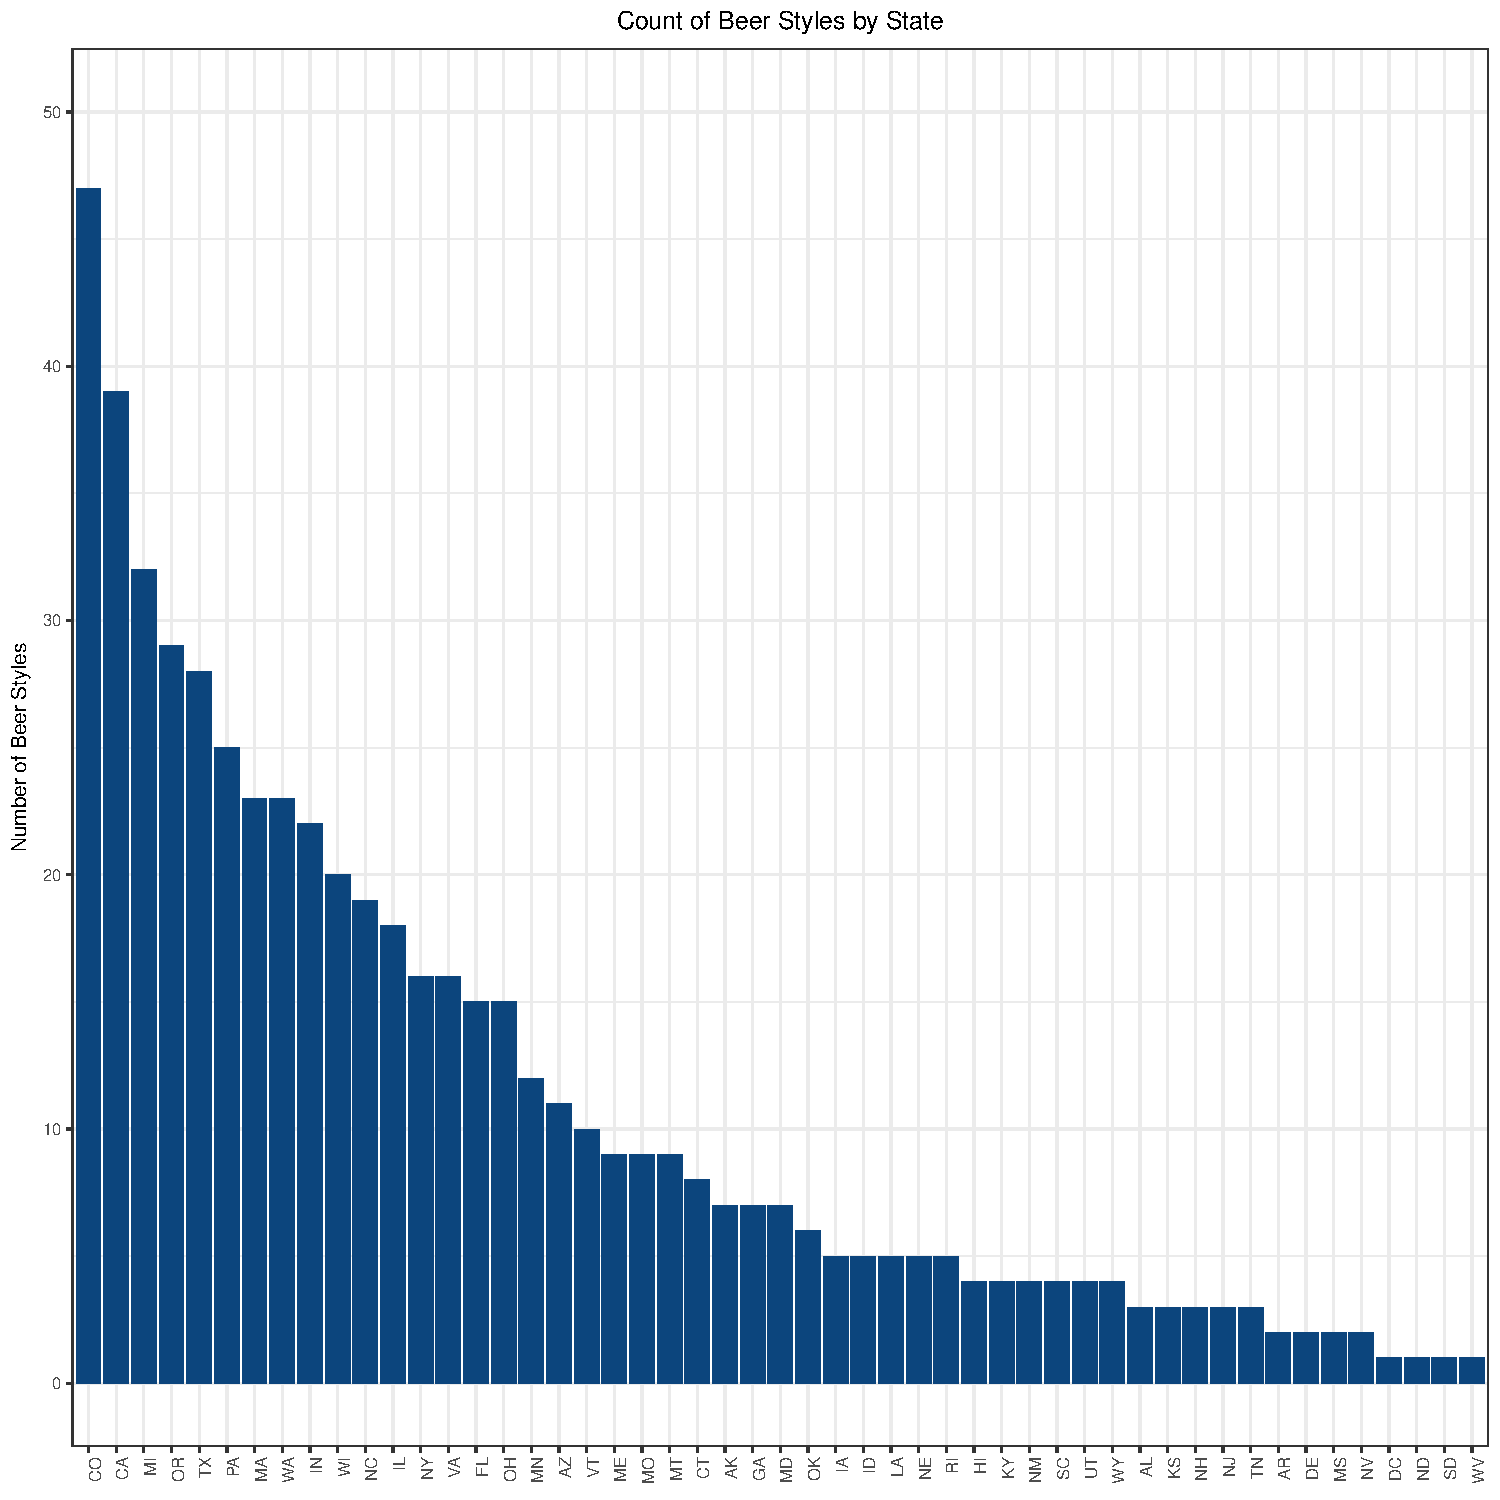
\includegraphics{Analysis_Final_files/figure-latex/unnamed-chunk-3-1} \end{center}

\subsubsection{Clean Breweries Data}\label{clean-breweries-data}

Before we can confidently proceed with our analysis it's important to
ensure we have scrubbed the data, removed duplicates, and decide how we
will deal with errors and missing values.

We start this process by removing punctuation and whitespace from
columns. Humans are fallible and typos are easy to make. Without knowing
the origin of the data in the files provided, its prudent to assume that
mistakes have been made and take measures to correct them.

Remvoing punctuation allows us to mitigate the possibility of commas
being erroneously typed as periods. ``Detroit, MI'', for example, would
be identified as a different city than ``Detroit. MI'' Removing
punctuation resolves this issue. Both city/state combinations simply
become ``Detroit MI.''

Likewise, it's helpful to remove whitespace. Although whitespace can
appear ``invisible'' to the human eye, computers can ``see'' this space
as if it were a number or a letter.

We use the apply function to make these changes to every row in the
dataframe.

Removing duplicates is more of a challenge. Before we can remove
duplicates we need to confirm whether or not two rows are the same. We
identify duplicates by creating a unique key for each brewery that's a
combination of the brewery ID, city, and state.

De-duplicating in this case is a multi-step process. We start by
identifying brewery ids that show up more than once which indicate
possible duplicates. Further investigation determines whether or not
they are actually duplicates.

In addition to removing identifying and removing duplicates
programatically, we also need to correct a few entries manually. There
are some entries that are clearly mis-spelled and need to be addressed.

Once potential duplicates are identified and assigned temporary keys,
they are evaluated apart from the main dataset and returned to the main
dataset once duplicates have been removed.

\begin{enumerate}
\def\labelenumi{\arabic{enumi})}
\tightlist
\item
  Remove punctuation and trim whitespace
\end{enumerate}

\begin{Shaded}
\begin{Highlighting}[]
\CommentTok{# remove punctionation from all columns and trim whitespace}
\NormalTok{breweries_data <-}\StringTok{ }\KeywordTok{as.data.frame}\NormalTok{(}
                      \KeywordTok{apply}\NormalTok{(breweries_data }\CommentTok{#data set}
\NormalTok{                            , }\DecValTok{2} \CommentTok{#apply function column-wise}
\NormalTok{                            , }\ControlFlowTok{function}\NormalTok{(x) }\KeywordTok{trimws}\NormalTok{(}\KeywordTok{gsub}\NormalTok{(}\StringTok{'[[:punct:] ]+'}\NormalTok{,}\StringTok{' '}\NormalTok{,x))) }\CommentTok{#anonymous function to remove punctuation and trim whitespace}
\NormalTok{                            , }\DataTypeTok{stringsAsFactors =} \OtherTok{FALSE}\NormalTok{)  }\CommentTok{#do not implicitly convert strings to factors}


\NormalTok{breweries_clean <-}\StringTok{ }\KeywordTok{distinct}\NormalTok{(breweries_data, brewery_id, }\DataTypeTok{.keep_all =} \OtherTok{TRUE}\NormalTok{) }\OperatorTok\StringTok{ }\KeywordTok{rename}\NormalTok{(}\DataTypeTok{brewery_name =}\NormalTok{ name) }\CommentTok{# select distinct breweries according to the unique composite key and rename}
\end{Highlighting}
\end{Shaded}

\begin{enumerate}
\def\labelenumi{\arabic{enumi})}
\setcounter{enumi}{1}
\tightlist
\item
  Configure column types
\end{enumerate}

\begin{Shaded}
\begin{Highlighting}[]
\NormalTok{breweries_data}\OperatorTok{$}\NormalTok{name <-}\StringTok{ }\KeywordTok{as.factor}\NormalTok{(breweries_data}\OperatorTok{$}\NormalTok{name) }\CommentTok{# convert Name column to factor}
\NormalTok{breweries_data}\OperatorTok{$}\NormalTok{brewery_id <-}\StringTok{ }\KeywordTok{as.integer}\NormalTok{(breweries_data}\OperatorTok{$}\NormalTok{brewery_id) }\CommentTok{# convert Brew_ID to integer}
\end{Highlighting}
\end{Shaded}

\begin{enumerate}
\def\labelenumi{\arabic{enumi})}
\setcounter{enumi}{2}
\tightlist
\item
  Identify and capture potential duplicate records
\end{enumerate}

\begin{Shaded}
\begin{Highlighting}[]
\CommentTok{# confirm Brew_ID + City + State is a unique key}
\NormalTok{breweries_summary <-}\StringTok{ }
\StringTok{  }\KeywordTok{select}\NormalTok{(breweries_data, brewery_id, city, state, name) }\OperatorTok
\StringTok{  }\KeywordTok{group_by}\NormalTok{(name) }\OperatorTok
\StringTok{  }\KeywordTok{summarize_all}\NormalTok{(}\KeywordTok{funs}\NormalTok{(}
    \DataTypeTok{count =} \KeywordTok{n_distinct}\NormalTok{(brewery_id, city, state))) }\OperatorTok
\StringTok{  }\KeywordTok{select}\NormalTok{(name, brewery_id_count) }\OperatorTok\StringTok{ }\CommentTok{# select only Name and Brew_ID_count columns}
\StringTok{  }\KeywordTok{arrange}\NormalTok{(}\KeywordTok{desc}\NormalTok{(brewery_id_count)) }\CommentTok{# sort by Brew_ID_count desc}
 

\CommentTok{# capture potential duplicates}
\NormalTok{breweries_dups <-}\StringTok{ }\KeywordTok{filter}\NormalTok{(breweries_summary, brewery_id_count }\OperatorTok{>}\StringTok{ }\DecValTok{1}\NormalTok{) }\CommentTok{# if Brew_ID_count > 1 then there is a potential duplicate on that Brew_ID}

\CommentTok{# rejoin potential dups to original dataset}
\NormalTok{breweries_dups <-}\StringTok{ }\KeywordTok{select}\NormalTok{(breweries_dups }\OperatorTok\StringTok{ }\KeywordTok{inner_join}\NormalTok{(breweries_data, }\DataTypeTok{by=}\StringTok{"name"}\NormalTok{), }\OperatorTok{-}\KeywordTok{ends_with}\NormalTok{(}\StringTok{"_count"}\NormalTok{))}

\KeywordTok{kable}\NormalTok{(breweries_dups)}
\end{Highlighting}
\end{Shaded}

\begin{longtable}[]{@{}lrll@{}}
\toprule
name & brewery\_id & city & state\tabularnewline
\midrule
\endhead
Blackrocks Brewery & 13 & Marquette & MI\tabularnewline
Blackrocks Brewery & 96 & Marquette & MA\tabularnewline
Blue Mountain Brewery & 383 & Afton & VA\tabularnewline
Blue Mountain Brewery & 415 & Arrington & VA\tabularnewline
Lucette Brewing Company & 378 & Menominee & WI\tabularnewline
Lucette Brewing Company & 457 & Menominie & WI\tabularnewline
Oskar Blues Brewery & 167 & Longmont & CO\tabularnewline
Oskar Blues Brewery & 504 & Lyons & CO\tabularnewline
Otter Creek Brewing & 262 & Waterbury & VT\tabularnewline
Otter Creek Brewing & 276 & Middlebury & VT\tabularnewline
Sly Fox Brewing Company & 164 & Phoenixville & PA\tabularnewline
Sly Fox Brewing Company & 372 & Pottstown & PA\tabularnewline
Summit Brewing Company & 59 & St Paul & MN\tabularnewline
Summit Brewing Company & 139 & St Paul & MN\tabularnewline
\bottomrule
\end{longtable}

\begin{enumerate}
\def\labelenumi{\arabic{enumi})}
\setcounter{enumi}{3}
\item
  Correct duplicates

  \begin{itemize}
  \tightlist
  \item
    City name ``Menominie'' misspelled as ``Menominee''
  \end{itemize}
\end{enumerate}

\begin{Shaded}
\begin{Highlighting}[]
\CommentTok{# Fix Brew_ID=378, change City(Menominee -> Menominie) }
\NormalTok{breweries_dups <-}\StringTok{ }\NormalTok{breweries_dups }\OperatorTok
\StringTok{     }\KeywordTok{mutate}\NormalTok{(}\DataTypeTok{city=}\KeywordTok{replace}\NormalTok{(city, brewery_id}\OperatorTok{==}\DecValTok{378}\NormalTok{, }\StringTok{"Menominie"}\NormalTok{)) }\OperatorTok
\StringTok{     }\KeywordTok{as.data.frame}\NormalTok{()}
\end{Highlighting}
\end{Shaded}

\begin{verbatim}
+ Marquette is not a city name in Massachusetts. Changed to Michigan based on other records existing for Marquette, MI, in addition to validating the location of the city on Google Maps.
\end{verbatim}

\begin{Shaded}
\begin{Highlighting}[]
\CommentTok{# Fix Brew_ID=96, change State(MA -> MI)}
\NormalTok{breweries_dups <-}\StringTok{ }\NormalTok{breweries_dups }\OperatorTok
\StringTok{     }\KeywordTok{mutate}\NormalTok{(}\DataTypeTok{state=}\KeywordTok{replace}\NormalTok{(state, brewery_id}\OperatorTok{==}\DecValTok{96}\NormalTok{, }\StringTok{"MI"}\NormalTok{)) }\OperatorTok
\StringTok{     }\KeywordTok{as.data.frame}\NormalTok{()}
\end{Highlighting}
\end{Shaded}

\begin{verbatim}
+ Merge duplicates into single records on name + city + state
\end{verbatim}

\begin{Shaded}
\begin{Highlighting}[]
\CommentTok{# group corrected duplicates to }
\NormalTok{breweries_dups <-}\StringTok{ }\NormalTok{breweries_dups }\OperatorTok
\StringTok{                  }\KeywordTok{group_by}\NormalTok{(name, city, state) }\OperatorTok
\StringTok{                  }\KeywordTok{filter}\NormalTok{(}\KeywordTok{n}\NormalTok{()}\OperatorTok{>}\DecValTok{1}\NormalTok{)}
\end{Highlighting}
\end{Shaded}

\begin{verbatim}
+ Create new brewery_id for corrected duplicates
\end{verbatim}

\begin{Shaded}
\begin{Highlighting}[]
\CommentTok{# create surrogate keys for duplicates}
\NormalTok{breweries_sk <-}\StringTok{ }\NormalTok{breweries_dups }\OperatorTok
\StringTok{                    }\KeywordTok{group_by}\NormalTok{(name, city, state) }\OperatorTok
\StringTok{                    }\KeywordTok{summarize_all}\NormalTok{(}\KeywordTok{funs}\NormalTok{(}
                        \DataTypeTok{brew_sk =}\NormalTok{ (}\KeywordTok{sum}\NormalTok{(brewery_id)}\OperatorTok{*}\KeywordTok{sum}\NormalTok{(brewery_id)),}
                        \DataTypeTok{count =} \KeywordTok{n}\NormalTok{()}
\NormalTok{                        )) }\OperatorTok
\StringTok{                    }\KeywordTok{ungroup}\NormalTok{() }\OperatorTok
\StringTok{                    }\KeywordTok{right_join}\NormalTok{(breweries_dups, }\DataTypeTok{by =} \KeywordTok{c}\NormalTok{(}\StringTok{"name"}\NormalTok{, }\StringTok{"city"}\NormalTok{, }\StringTok{"state"}\NormalTok{)) }\OperatorTok\StringTok{ }\CommentTok{# rejoin to dupes by name, city, state}
\StringTok{                    }\KeywordTok{rename}\NormalTok{(}\DataTypeTok{old_brewery_id=}\NormalTok{brewery_id, }\DataTypeTok{new_brewery_id=}\NormalTok{brew_sk)}
              
  
\KeywordTok{kable}\NormalTok{(breweries_sk)}
\end{Highlighting}
\end{Shaded}

\begin{longtable}[]{@{}lllrrr@{}}
\toprule
name & city & state & new\_brewery\_id & count &
old\_brewery\_id\tabularnewline
\midrule
\endhead
Blackrocks Brewery & Marquette & MI & 11881 & 2 & 13\tabularnewline
Blackrocks Brewery & Marquette & MI & 11881 & 2 & 96\tabularnewline
Lucette Brewing Company & Menominie & WI & 697225 & 2 &
378\tabularnewline
Lucette Brewing Company & Menominie & WI & 697225 & 2 &
457\tabularnewline
Summit Brewing Company & St Paul & MN & 39204 & 2 & 59\tabularnewline
Summit Brewing Company & St Paul & MN & 39204 & 2 & 139\tabularnewline
\bottomrule
\end{longtable}

\begin{verbatim}
+ Update original breweries dataset with corrections and de-duped records
\end{verbatim}

\begin{Shaded}
\begin{Highlighting}[]
\CommentTok{# create cleaned dataset}

\NormalTok{breweries_clean <-}\StringTok{ }\NormalTok{dplyr}\OperatorTok{::}\KeywordTok{bind_rows}\NormalTok{( }\CommentTok{# append rows of dataframes together}
\NormalTok{                          breweries_data }\OperatorTok\StringTok{ }
\StringTok{                            }\KeywordTok{filter}\NormalTok{(}\OperatorTok{!}\NormalTok{brewery_id }\OperatorTok\StringTok{ }\NormalTok{breweries_sk}\OperatorTok{$}\NormalTok{old_brewery_id), }\CommentTok{# remove duplicated records from breweries_data}
\NormalTok{                          breweries_sk }\OperatorTok\StringTok{ }
\StringTok{                            }\KeywordTok{rename}\NormalTok{(}\DataTypeTok{brewery_id=}\NormalTok{new_brewery_id) }\OperatorTok\StringTok{ }\CommentTok{# rename new_brewery_id to brewery_id so the rbind works}
\StringTok{                            }\KeywordTok{select}\NormalTok{(}\OperatorTok{-}\NormalTok{count, }\OperatorTok{-}\NormalTok{old_brewery_id)) }\OperatorTok\StringTok{ }\CommentTok{# remove extra columns from brewery_sk data frame}
\StringTok{                          }\KeywordTok{rename}\NormalTok{(}\DataTypeTok{brewery_name =}\NormalTok{ name) }\OperatorTok\StringTok{ }\CommentTok{#change column name "name" to "brewery_name"}
\StringTok{                          }\KeywordTok{mutate}\NormalTok{(}\DataTypeTok{state =} \KeywordTok{as.factor}\NormalTok{(state))}

\KeywordTok{print}\NormalTok{(summarytools}\OperatorTok{::}\KeywordTok{dfSummary}\NormalTok{(breweries_clean), }\DataTypeTok{method =} \StringTok{'render'}\NormalTok{)}
\end{Highlighting}
\end{Shaded}

Data Frame Summary

breweries\_clean

N: 558

\begin{verbatim}
<tr>
  <th align="center"><strong>No</strong></th>
  <th align="center"><strong>Variable</strong></th>
  <th align="center"><strong>Stats / Values</strong></th>
  <th align="center"><strong>Freqs (% of Valid)</strong></th>
  <th align="center"><strong>Graph</strong></th>
  <th align="center"><strong>Valid</strong></th>
  <th align="center"><strong>Missing</strong></th>
</tr>
\end{verbatim}

\begin{verbatim}
<tr>
  <td align="center">1</td>
  <td align="left">brewery_id
\end{verbatim}

{[}integer{]}

\begin{verbatim}
  <td align="left">mean (sd) : 2959.57 (41747.55)
\end{verbatim}

min \textless{} med \textless{} max : 1 \textless{} 283.5 \textless{}
697225 IQR (CV) : 279.5 (14.11)

\begin{verbatim}
  <td align="left">555 distinct val.</td>
  <td align="center" border="0"><img src="data:image/png;base64,iVBORw0KGgoAAAANSUhEUgAAAJYAAABkCAMAAABThTnCAAAADFBMVEX9/v2mpqby8vL9/v28xacEAAAABHRSTlP///8AQCqp9AAAAJNJREFUaIHt27ENgzAAAEET9t+ZIiAiBSF9ZRd3E/wCP/YljdkBz2QV36ztNrnndGZ9LrLeyCpkFbIKWYWsQlYhq5BVyCpkFbIKWYWsQlYhq5BVyCpkFbIKWYWsQlYhq5BVyCpkFbIKWYWsQlYhq5BVyCpkFbIKWYWsQlYhq5BVyCpkFbIKWcXfrDXdT9ZyZBWLZh3aJKoJ7TmyggAAAABJRU5ErkJggg=="></td>
  <td align="center">558
\end{verbatim}

(100\%)

\begin{verbatim}
  <td align="center">0
\end{verbatim}

(0\%)

\begin{verbatim}
</tr>
<tr>
  <td align="center">2</td>
  <td align="left">brewery_name
\end{verbatim}

{[}factor{]}

\begin{verbatim}
  <td align="left">1. 10 Barrel Brewing Company
\end{verbatim}

\begin{enumerate}
\def\labelenumi{\arabic{enumi}.}
\setcounter{enumi}{1}
\tightlist
\item
  18th Street Brewery
\item
  2 Towns Ciderhouse
\item
  21st Amendment Brewery
\item
  3 Daughters Brewing
\item
  4 Hands Brewing Company
\item
  450 North Brewing Company
\item
  7 Seas Brewing Company
\item
  7venth Sun
\item
  Abita Brewing Company {[} 541 others {]}

  1 (0.2\%) 1 (0.2\%) 1 (0.2\%) 1 (0.2\%) 1 (0.2\%) 1 (0.2\%) 1 (0.2\%)
  1 (0.2\%) 1 (0.2\%) 1 (0.2\%) 548 (98.6\%)

  558 (100\%)

  0 (0\%)

  3

  city {[}character{]}

  \begin{enumerate}
  \def\labelenumii{\arabic{enumii}.}
  \tightlist
  \item
    Portland
  \end{enumerate}
\item
  Boulder
\item
  Chicago
\item
  Seattle
\item
  Austin
\item
  Denver
\item
  San Diego
\item
  Bend
\item
  San Francisco
\item
  Anchorage {[} 372 others {]}

  17 (3.0\%) 9 (1.6\%) 9 (1.6\%) 9 (1.6\%) 8 (1.4\%) 8 (1.4\%) 8 (1.4\%)
  6 (1.1\%) 5 (0.9\%) 4 (0.7\%) 475 (85.5\%)

  558 (100\%)

  0 (0\%)

  4

  state {[}factor{]}

  \begin{enumerate}
  \def\labelenumii{\arabic{enumii}.}
  \tightlist
  \item
    AK
  \end{enumerate}
\item
  AL
\item
  AR
\item
  AZ
\item
  CA
\item
  CO
\item
  CT
\item
  DC
\item
  DE
\item
  FL {[} 41 others {]}

  7 (1.2\%) 3 (0.5\%) 2 (0.4\%) 11 (2.0\%) 39 (7.0\%) 47 (8.4\%) 8
  (1.4\%) 1 (0.2\%) 2 (0.4\%) 15 (2.7\%) 423 (75.8\%)

  558 (100\%)

  0 (0\%)

  Generated by summarytools 0.8.5 (R version 3.5.0)2018-06-26
\end{enumerate}

\subsection{Clean Beer Data}\label{clean-beer-data}

A similar process is used to remove duplicates from the Beers dataset.

\begin{Shaded}
\begin{Highlighting}[]
\NormalTok{beer_data <-}\StringTok{ }\KeywordTok{read.csv}\NormalTok{(}\StringTok{"../data/Beers.csv"}\NormalTok{, }\DataTypeTok{header=}\OtherTok{TRUE}\NormalTok{)}

\KeywordTok{head}\NormalTok{(beer_data)}
\end{Highlighting}
\end{Shaded}

\begin{verbatim}
             Name Beer_ID   ABV IBU Brewery_id
\end{verbatim}

1 Pub Beer 1436 0.050 NA 409 2 Devil's Cup 2265 0.066 NA 178 3 Rise of
the Phoenix 2264 0.071 NA 178 4 Sinister 2263 0.090 NA 178 5 Sex and
Candy 2262 0.075 NA 178 6 Black Exodus 2261 0.077 NA 178 Style Ounces 1
American Pale Lager 12 2 American Pale Ale (APA) 12 3 American IPA 12 4
American Double / Imperial IPA 12 5 American IPA 12 6 Oatmeal Stout 12

\begin{Shaded}
\begin{Highlighting}[]
\KeywordTok{nrow}\NormalTok{(beer_data)}
\end{Highlighting}
\end{Shaded}

{[}1{]} 2410

\begin{Shaded}
\begin{Highlighting}[]
\KeywordTok{colnames}\NormalTok{(beer_data) }\OperatorTok\StringTok{ }\NormalTok{tolower }\CommentTok{#lower case colnames}





\NormalTok{beer_clean <-}\StringTok{ }\KeywordTok{merge}\NormalTok{(beer_data, }\CommentTok{# first data frame}
\NormalTok{             (breweries_sk }\OperatorTok\StringTok{ }\KeywordTok{select}\NormalTok{(old_brewery_id, new_brewery_id)), }\CommentTok{# second data frame}
             \DataTypeTok{by.x =} \StringTok{"brewery_id"}\NormalTok{, }\CommentTok{# left table join key}
             \DataTypeTok{by.y =} \StringTok{"old_brewery_id"}\NormalTok{, }\CommentTok{# right table join key}
             \DataTypeTok{all =}\NormalTok{ T) }\OperatorTok\StringTok{ }\CommentTok{# keep all columns}
\StringTok{       }\KeywordTok{mutate}\NormalTok{(}\DataTypeTok{brewery_id =} \KeywordTok{ifelse}\NormalTok{(}\OperatorTok{!}\KeywordTok{is.na}\NormalTok{(new_brewery_id), new_brewery_id, brewery_id)) }\OperatorTok\StringTok{  }\CommentTok{# update brewery_id with new_brewery_id, if new_brewery_id is not null}
\StringTok{       }\KeywordTok{select}\NormalTok{(}\OperatorTok{-}\NormalTok{new_brewery_id) }\OperatorTok\StringTok{ }\CommentTok{# drop new_brewery_id column}
\StringTok{       }\KeywordTok{rename}\NormalTok{(}\DataTypeTok{beer_name =}\NormalTok{ name)}


\KeywordTok{print}\NormalTok{(summarytools}\OperatorTok{::}\KeywordTok{dfSummary}\NormalTok{(beer_clean), }\DataTypeTok{method =} \StringTok{'render'}\NormalTok{)}
\end{Highlighting}
\end{Shaded}

Data Frame Summary

beer\_clean

N: 2410

\begin{verbatim}
<tr>
  <th align="center"><strong>No</strong></th>
  <th align="center"><strong>Variable</strong></th>
  <th align="center"><strong>Stats / Values</strong></th>
  <th align="center"><strong>Freqs (% of Valid)</strong></th>
  <th align="center"><strong>Graph</strong></th>
  <th align="center"><strong>Valid</strong></th>
  <th align="center"><strong>Missing</strong></th>
</tr>
\end{verbatim}

\begin{verbatim}
<tr>
  <td align="center">1</td>
  <td align="left">brewery_id
\end{verbatim}

{[}integer{]}

\begin{verbatim}
  <td align="left">mean (sd) : 1488.62 (28425.37)
\end{verbatim}

min \textless{} med \textless{} max : 1 \textless{} 207 \textless{}
697225 IQR (CV) : 273.5 (19.1)

\begin{verbatim}
  <td align="left">555 distinct val.</td>
  <td align="center" border="0"><img src="data:image/png;base64,iVBORw0KGgoAAAANSUhEUgAAAJYAAABkCAMAAABThTnCAAAADFBMVEX9/v2mpqby8vL9/v28xacEAAAABHRSTlP///8AQCqp9AAAAJNJREFUaIHt27ENgzAAAEET9t+ZIiAiBSF9ZRd3E/wCP/YljdkBz2QV36ztNrnndGZ9LrLeyCpkFbIKWYWsQlYhq5BVyCpkFbIKWYWsQlYhq5BVyCpkFbIKWYWsQlYhq5BVyCpkFbIKWYWsQlYhq5BVyCpkFbIKWYWsQlYhq5BVyCpkFbIKWcXfrDXdT9ZyZBWLZh3aJKoJ7TmyggAAAABJRU5ErkJggg=="></td>
  <td align="center">2410
\end{verbatim}

(100\%)

\begin{verbatim}
  <td align="center">0
\end{verbatim}

(0\%)

\begin{verbatim}
</tr>
<tr>
  <td align="center">2</td>
  <td align="left">beer_name
\end{verbatim}

{[}factor{]}

\begin{verbatim}
  <td align="left">1. #001 Golden Amber Lager
\end{verbatim}

\begin{enumerate}
\def\labelenumi{\arabic{enumi}.}
\setcounter{enumi}{1}
\item ~
  \section{002 American I.P.A.}\label{american-i.p.a.}
\item ~
  \section{003 Brown \& Robust Porte}\label{brown-robust-porte}
\item ~
  \section{004 Session I.P.A.}\label{session-i.p.a.}
\item ~
  \section{9}\label{section}
\item
  077XX
\item
  10 Degrees of Separation
\item
  10 Ton
\item
  113 IPA
\item
  11th Hour IPA {[} 2295 others {]}

  1 (0.0\%) 1 (0.0\%) 1 (0.0\%) 1 (0.0\%) 2 (0.1\%) 1 (0.0\%) 1 (0.0\%)
  1 (0.0\%) 1 (0.0\%) 1 (0.0\%) 2399 (96.0\%)

  2410 (100\%)

  0 (0\%)

  3

  beer\_id {[}integer{]}

  mean (sd) : 1431.11 (752.46) min \textless{} med \textless{} max : 1
  \textless{} 1453.5 \textless{} 2692 IQR (CV) : 1267.5 (0.53)

  2410 distinct val.

  2410 (100\%)

  0 (0\%)

  4

  abv {[}numeric{]}

  mean (sd) : 0.06 (0.01) min \textless{} med \textless{} max : 0
  \textless{} 0.06 \textless{} 0.13 IQR (CV) : 0.02 (0.23)

  74 distinct val.

  2348 (97.43\%)

  62 (2.57\%)

  5

  ibu {[}integer{]}

  mean (sd) : 42.71 (25.95) min \textless{} med \textless{} max : 4
  \textless{} 35 \textless{} 138 IQR (CV) : 43 (0.61)

  107 distinct val.

  1405 (58.3\%)

  1005 (41.7\%)

  6

  style {[}factor{]}

  \begin{enumerate}
  \def\labelenumii{\arabic{enumii}.}
  \item
  \end{enumerate}
\item
  Abbey Single Ale
\item
  Altbier
\item
  American Adjunct Lager
\item
  American Amber / Red Ale
\item
  American Amber / Red Lage
\item
  American Barleywine
\item
  American Black Ale
\item
  American Blonde Ale
\item
  American Brown Ale {[} 90 others {]}

  5 (0.2\%) 2 (0.1\%) 13 (0.5\%) 18 (0.8\%) 133 (5.5\%) 29 (1.2\%) 3
  (0.1\%) 36 (1.5\%) 108 (4.5\%) 70 (2.9\%) 1993 (82.7\%)

  2410 (100\%)

  0 (0\%)

  7

  ounces {[}numeric{]}

  mean (sd) : 13.59 (2.35) min \textless{} med \textless{} max : 8.4
  \textless{} 12 \textless{} 32 IQR (CV) : 4 (0.17)

  8.40 : 1 (0.0\%) 12.00 : 1525 (63.3\%) 16.00 : 841 (34.9\%) 16.90 : 1
  (0.0\%) 19.20 : 15 (0.6\%) 24.00 : 22 (0.9\%) 32.00 : 5 (0.2\%)

  2410 (100\%)

  0 (0\%)

  Generated by summarytools 0.8.5 (R version 3.5.0)2018-06-26
\end{enumerate}

\subsection{Question 1}\label{question-1}

To determine the number breweries in each state we simply count the
number of times each state appears in the table.

The prominent brewing states with twenty or more breweries include:
Colorado 47, California 39, Michigan 32, Oregon 29, Texas 28,
Pennsylvania 25, Massachusetts 23, Washington 23, Indiana 22, Wisconsin
20.

These prominent brewing states are important to the beer market, because
of their distinct beer types and styles that are produced in state and
consumed nationally.

What kinds of beers and their characteristics will be of great interest
for the analysis.

\begin{Shaded}
\begin{Highlighting}[]
\CommentTok{#TODO: break up chunk}

\NormalTok{state_ll <-}\StringTok{ }\KeywordTok{read.csv}\NormalTok{(}\StringTok{"../data/state_coords.csv"}\NormalTok{) }\OperatorTok\StringTok{ }
\StringTok{                    }\KeywordTok{mutate}\NormalTok{(}\DataTypeTok{State =} \KeywordTok{toupper}\NormalTok{(State)) }\OperatorTok\StringTok{ }
\StringTok{                    }\KeywordTok{rename}\NormalTok{(}\DataTypeTok{name =}\NormalTok{ State, }\DataTypeTok{lat_center =}\NormalTok{ Latitude, }\DataTypeTok{lon_center =}\NormalTok{ Longitude)}
        

\NormalTok{states <-}\StringTok{ }\KeywordTok{map_data}\NormalTok{(}\StringTok{"state"}\NormalTok{) }\OperatorTok
\StringTok{          }\KeywordTok{mutate}\NormalTok{(}\DataTypeTok{region =} \KeywordTok{toupper}\NormalTok{(region)) }\OperatorTok
\StringTok{          }\KeywordTok{rename}\NormalTok{(}\DataTypeTok{name=}\NormalTok{region) }\OperatorTok
\StringTok{          }\KeywordTok{select}\NormalTok{(long, lat, name, group)}
 
\CommentTok{# states %>% group_by(name) %>%}
\CommentTok{#             summarise_all(funs(n=n()))}
\CommentTok{# }
\CommentTok{#        }
\NormalTok{states <-}\StringTok{ }\NormalTok{states }\OperatorTok\StringTok{          }
\StringTok{          }\KeywordTok{left_join}\NormalTok{(}
\NormalTok{            states }\OperatorTok
\StringTok{            }\KeywordTok{group_by}\NormalTok{(name) }\OperatorTok
\StringTok{            }\KeywordTok{summarise_all}\NormalTok{(}\KeywordTok{funs}\NormalTok{(}\DataTypeTok{n=}\KeywordTok{n}\NormalTok{())) }\OperatorTok
\StringTok{            }\KeywordTok{select}\NormalTok{(name, group_n) }\OperatorTok
\StringTok{            }\KeywordTok{distinct}\NormalTok{(name, }\DataTypeTok{.keep_all =} \OtherTok{TRUE}\NormalTok{)}
\NormalTok{          )}
          
          



\NormalTok{breweries_by_state <-}\StringTok{ }\KeywordTok{select}\NormalTok{(breweries_clean, brewery_id, state) }\OperatorTok
\StringTok{  }\KeywordTok{group_by}\NormalTok{(state) }\OperatorTok
\StringTok{  }\KeywordTok{summarise_all}\NormalTok{(}\KeywordTok{funs}\NormalTok{(}\DataTypeTok{brewery_count =} \KeywordTok{n}\NormalTok{()))  }\OperatorTok
\StringTok{  }\KeywordTok{left_join}\NormalTok{(state_ll, }\DataTypeTok{by=}\KeywordTok{c}\NormalTok{(}\StringTok{"state"}\NormalTok{ =}\StringTok{ "Abbr"}\NormalTok{))}


\CommentTok{# state_ll %>%}
\CommentTok{#   inner_join(states)}



\NormalTok{summarytools}\OperatorTok{::}\KeywordTok{dfSummary}\NormalTok{(breweries_by_state, }\DataTypeTok{transpose =} \OtherTok{TRUE}\NormalTok{)}
\end{Highlighting}
\end{Shaded}

Data Frame Summary\\
breweries\_by\_state\\
N: 51\\
------------------------------------------------------------------------------------------------------------------------------------
No Variable Stats / Values Freqs (\% of Valid) Text Graph Valid
Missing\\
---- ---------------- ----------------------------- --------------------
-------------------------------------- ---------- --------- 1 state 1.
AK 1 ( 2.0\%) 51 0\\
{[}character{]} 2. AL 1 ( 2.0\%) (100\%) (0\%)\\
3. AR 1 ( 2.0\%)\\
4. AZ 1 ( 2.0\%)\\
5. CA 1 ( 2.0\%)\\
6. CO 1 ( 2.0\%)\\
7. CT 1 ( 2.0\%)\\
8. DC 1 ( 2.0\%)\\
9. DE 1 ( 2.0\%)\\
10. FL 1 ( 2.0\%)\\
{[} 41 others {]} 41 (80.4\%) IIIIIIIIIIIIIIII

2 brewery\_count mean (sd) : 10.94 (10.63) 25 distinct val. : 51 0\\
{[}integer{]} min \textless{} med \textless{} max : : (100\%) (0\%)\\
1 \textless{} 7 \textless{} 47 :\\
IQR (CV) : 12.5 (0.97) : :\\
: : . : : . .

3 name 1. ALABAMA 1 ( 2.0\%) 50 1\\
{[}character{]} 2. ALASKA 1 ( 2.0\%) (98.04\%) (1.96\%)\\
3. ARIZONA 1 ( 2.0\%)\\
4. ARKANSAS 1 ( 2.0\%)\\
5. CALIFORNIA 1 ( 2.0\%)\\
6. COLORADO 1 ( 2.0\%)\\
7. CONNECTICUT 1 ( 2.0\%)\\
8. DELAWARE 1 ( 2.0\%)\\
9. FLORIDA 1 ( 2.0\%)\\
10. GEORGIA 1 ( 2.0\%)\\
{[} 40 others {]} 40 (80.0\%) IIIIIIIIIIIIIIII

4 lat\_center mean (sd) : 39.48 (6.13) 50 distinct val. : 50 1\\
{[}numeric{]} min \textless{} med \textless{} max : . : (98.04\%)
(1.96\%)\\
21.09 \textless{} 40 \textless{} 61.37 : :\\
IQR (CV) : 7.52 (0.16) : : :\\
: : : :

5 lon\_center mean (sd) : -93.67 (19.34) 50 distinct val. . : 50 1\\
{[}numeric{]} min \textless{} med \textless{} max : . : : (98.04\%)
(1.96\%)\\
-157.5 \textless{} -89.65 \textless{} -69.38 . . : : :\\
IQR (CV) : 23.84 (-0.21) : : : : : :\\
: : : : : : :\\
------------------------------------------------------------------------------------------------------------------------------------

\begin{Shaded}
\begin{Highlighting}[]
\CommentTok{#map of breweries by state}

\CommentTok{#one to many join of breweries by state}
\NormalTok{breweries_geo <-}\StringTok{ }\NormalTok{breweries_by_state }\OperatorTok
\StringTok{                  }\KeywordTok{inner_join}\NormalTok{(states, }\DataTypeTok{by =} \KeywordTok{c}\NormalTok{(}\StringTok{"name"}\NormalTok{ =}\StringTok{ "name"}\NormalTok{))}

\CommentTok{# map chart of brweeries_by_state}
\KeywordTok{ggplot}\NormalTok{((breweries_geo }\OperatorTok\StringTok{ }\KeywordTok{arrange}\NormalTok{(}\KeywordTok{desc}\NormalTok{(brewery_count))), }
       \KeywordTok{aes}\NormalTok{(}\DataTypeTok{group =}\NormalTok{ state, }\DataTypeTok{stat=}\StringTok{"identity"}\NormalTok{)) }\OperatorTok{+}
\StringTok{  }\KeywordTok{geom_polygon}\NormalTok{(}\KeywordTok{aes}\NormalTok{(}\DataTypeTok{x =}\NormalTok{ long, }
                   \DataTypeTok{y =}\NormalTok{ lat, }
                   \DataTypeTok{group=}\NormalTok{group, }
                   \DataTypeTok{fill=}\NormalTok{brewery_count), }
               \DataTypeTok{color =} \StringTok{"black"}\NormalTok{) }\OperatorTok{+}\StringTok{ }
\StringTok{  }\KeywordTok{geom_text}\NormalTok{(}\DataTypeTok{data =}\NormalTok{ (breweries_by_state }\OperatorTok\StringTok{ }
\StringTok{                    }\KeywordTok{filter}\NormalTok{(}\OperatorTok{!}\NormalTok{(state }\OperatorTok\StringTok{ }\KeywordTok{c}\NormalTok{(}\StringTok{"AK"}\NormalTok{, }\StringTok{"DC"}\NormalTok{, }\StringTok{"HI"}\NormalTok{)))), }\CommentTok{#filter to continental 50 states}
            \KeywordTok{aes}\NormalTok{(}\DataTypeTok{x =}\NormalTok{ lon_center, }
                \DataTypeTok{y =}\NormalTok{ lat_center, }
                \DataTypeTok{label =} \KeywordTok{as.character}\NormalTok{(brewery_count)),}
            \DataTypeTok{color =} \StringTok{'white'}
\NormalTok{            ) }\OperatorTok{+}
\StringTok{  }\KeywordTok{guides}\NormalTok{(}\DataTypeTok{fill=}\KeywordTok{guide_legend}\NormalTok{(}\DataTypeTok{title=} \StringTok{"Brewery Count"}\NormalTok{)) }\OperatorTok{+}
\StringTok{  }\KeywordTok{scale_fill_continuous}\NormalTok{(}\DataTypeTok{breaks =} \KeywordTok{seq}\NormalTok{(}\DecValTok{0}\NormalTok{,}\DecValTok{50}\NormalTok{, }\DataTypeTok{by =} \DecValTok{5}\NormalTok{)) }\OperatorTok{+}
\StringTok{  }\KeywordTok{coord_fixed}\NormalTok{(}\FloatTok{1.3}\NormalTok{) }\OperatorTok{+}\StringTok{ }\CommentTok{# fix lat/long display ratio}
\StringTok{  }
\StringTok{  }\KeywordTok{ggtitle}\NormalTok{(}\StringTok{"Breweries by State"}\NormalTok{) }\OperatorTok{+}\StringTok{ }\CommentTok{# set plot title}
\StringTok{  }\KeywordTok{theme}\NormalTok{(}\DataTypeTok{plot.title =} \KeywordTok{element_text}\NormalTok{(}\DataTypeTok{hjust =} \FloatTok{0.5}\NormalTok{)) }\OperatorTok{+}\StringTok{ }\CommentTok{# center plot title}
\StringTok{  }\KeywordTok{theme}\NormalTok{(}\DataTypeTok{legend.position =} \StringTok{"left"}\NormalTok{,}
        \DataTypeTok{axis.title.x=}\KeywordTok{element_blank}\NormalTok{(), }\CommentTok{# hide x axis title}
        \DataTypeTok{axis.text.x=}\KeywordTok{element_blank}\NormalTok{(),  }\CommentTok{# hide x axis text}
        \DataTypeTok{axis.ticks.x=}\KeywordTok{element_blank}\NormalTok{(), }\CommentTok{# hide x axis ticks}
        \DataTypeTok{axis.title.y=}\KeywordTok{element_blank}\NormalTok{(), }\CommentTok{# hide y axis title}
        \DataTypeTok{axis.text.y=}\KeywordTok{element_blank}\NormalTok{(),  }\CommentTok{# hide y axis text}
        \DataTypeTok{axis.ticks.y=}\KeywordTok{element_blank}\NormalTok{()) }\CommentTok{# hide y axis ticks}
\end{Highlighting}
\end{Shaded}

\begin{center}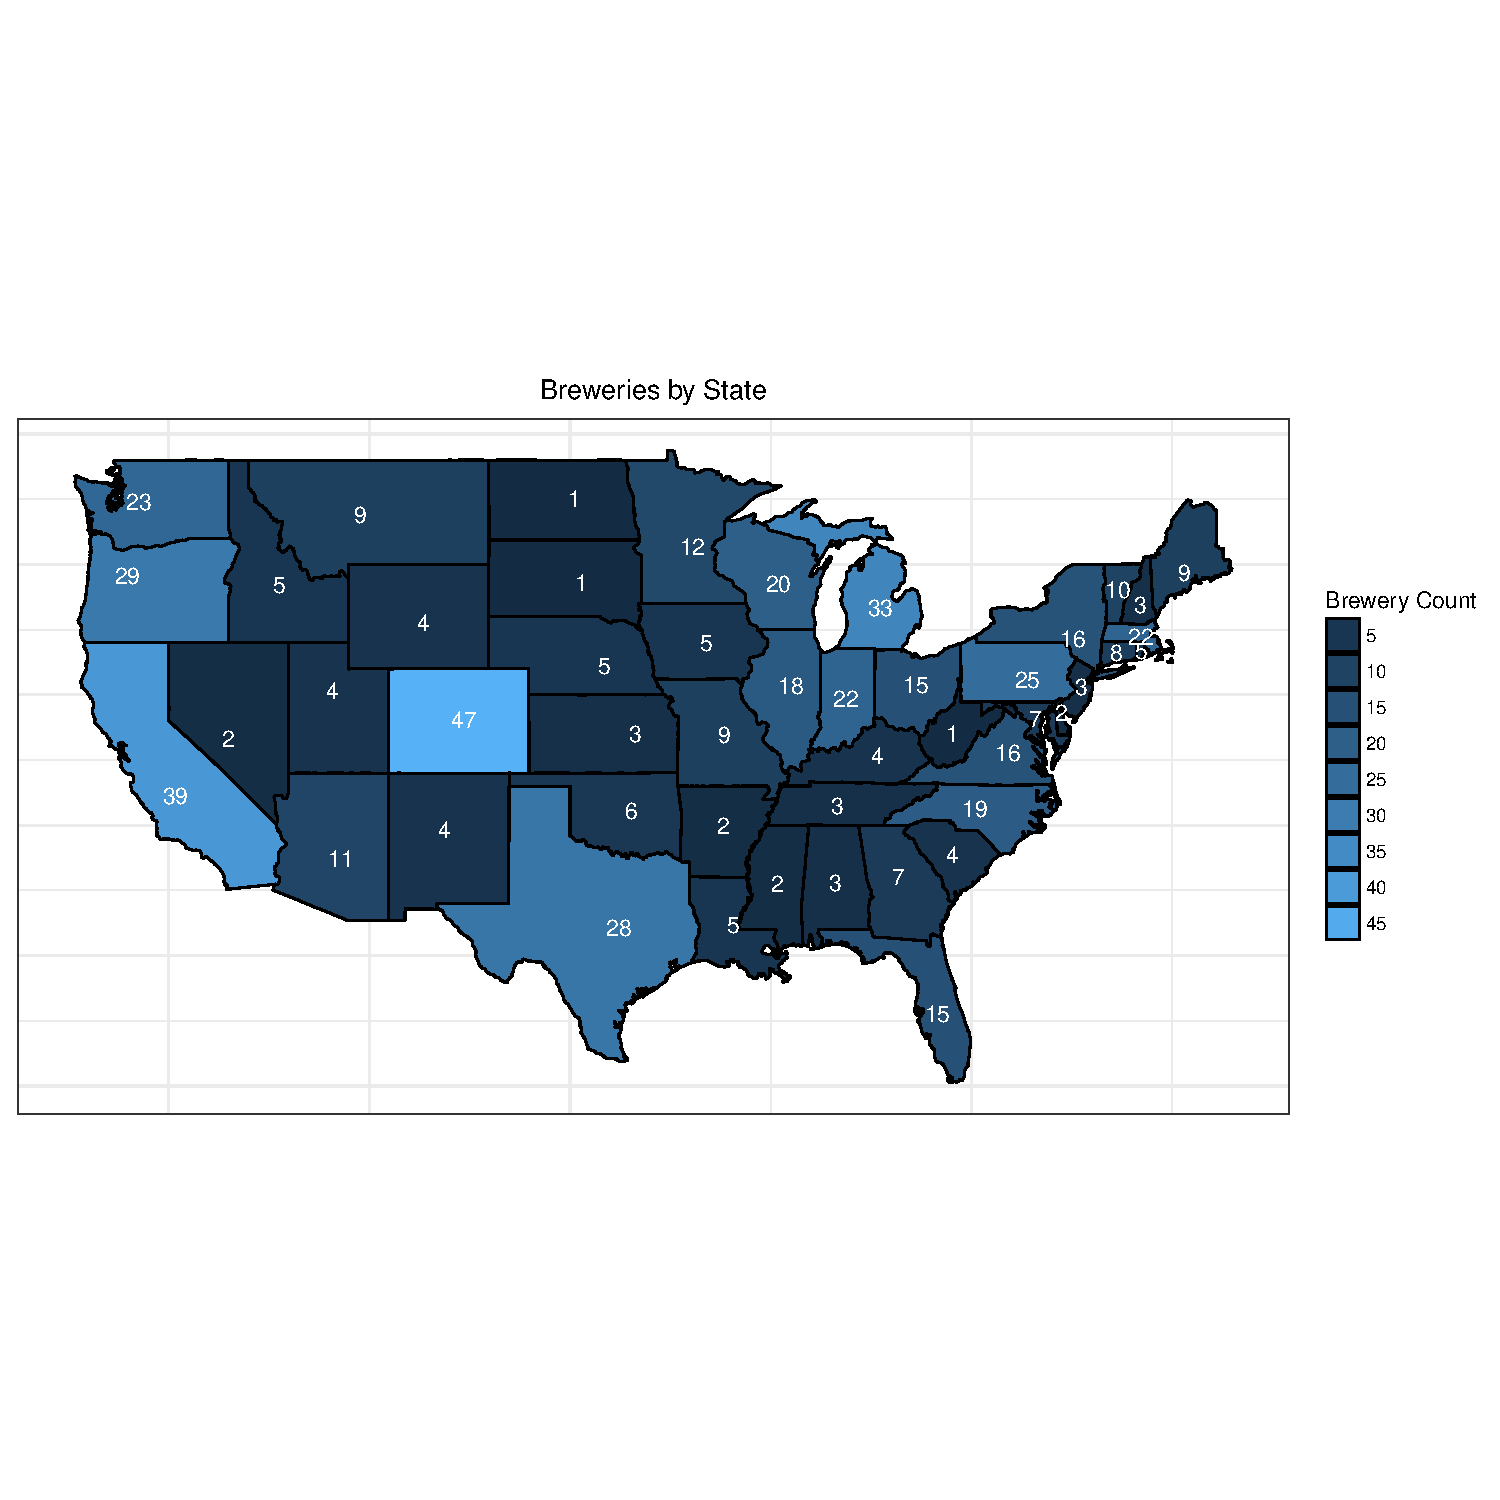
\includegraphics{Analysis_Final_files/figure-latex/unnamed-chunk-14-1} \end{center}

\subsection{Question 2}\label{question-2}

In data science, like in life, sometimes less is more. Instead of
maintaining separate tables for breweries and beers, it's helpful to
merge the two datasets into a single combined dataset.

We do this by joining the two tables by the Brew\_ID variable to create
a new object variable named merged\_data, which allows us to view the
desired characteristics of beers produced by the prominent breweries.

Those characteristics will be of high importance for the analysis of
most deisired beers, and we can begin to get clues of the prominent
beers when we programmatically arrange these data by the most frequent
style name variable sorted by every brewery.

\begin{Shaded}
\begin{Highlighting}[]
\CommentTok{# merge beer and breweries}
\NormalTok{merged_data <-}\StringTok{ }\NormalTok{breweries_clean }\OperatorTok
\StringTok{               }\KeywordTok{full_join}\NormalTok{(beer_clean, }\DataTypeTok{by=}\StringTok{"brewery_id"}\NormalTok{)}

\KeywordTok{kable}\NormalTok{(}\KeywordTok{head}\NormalTok{(merged_data, }\DecValTok{6}\NormalTok{), }\DataTypeTok{digits =} \DecValTok{2}\NormalTok{)}
\end{Highlighting}
\end{Shaded}

\begin{longtable}[]{@{}rllllrrrlr@{}}
\toprule
brewery\_id & brewery\_name & city & state & beer\_name & beer\_id & abv
& ibu & style & ounces\tabularnewline
\midrule
\endhead
1 & NorthGate Brewing & Minneapolis & MN & Get Together & 2692 & 0.04 &
50 & American IPA & 16\tabularnewline
1 & NorthGate Brewing & Minneapolis & MN & Maggie's Leap & 2691 & 0.05 &
26 & Milk / Sweet Stout & 16\tabularnewline
1 & NorthGate Brewing & Minneapolis & MN & Wall's End & 2690 & 0.05 & 19
& English Brown Ale & 16\tabularnewline
1 & NorthGate Brewing & Minneapolis & MN & Pumpion & 2689 & 0.06 & 38 &
Pumpkin Ale & 16\tabularnewline
1 & NorthGate Brewing & Minneapolis & MN & Stronghold & 2688 & 0.06 & 25
& American Porter & 16\tabularnewline
1 & NorthGate Brewing & Minneapolis & MN & Parapet ESB & 2687 & 0.06 &
47 & Extra Special / Strong Bitter (ESB) & 16\tabularnewline
\bottomrule
\end{longtable}

\begin{Shaded}
\begin{Highlighting}[]
\KeywordTok{kable}\NormalTok{(}\KeywordTok{tail}\NormalTok{(merged_data, }\DecValTok{6}\NormalTok{), }\DataTypeTok{digits =} \DecValTok{2}\NormalTok{)}
\end{Highlighting}
\end{Shaded}

\begin{longtable}[]{@{}lrllllrrrlr@{}}
\toprule
& brewery\_id & brewery\_name & city & state & beer\_name & beer\_id &
abv & ibu & style & ounces\tabularnewline
\midrule
\endhead
2420 & 39204 & Summit Brewing Company & St Paul & MN & Unchained \#18
Hop Silo & 2415 & 0.08 & 100 & American Double / Imperial IPA &
16\tabularnewline
2421 & 39204 & Summit Brewing Company & St Paul & MN & Extra Pale Ale &
2352 & 0.05 & 49 & American Pale Ale (APA) & 12\tabularnewline
2422 & 39204 & Summit Brewing Company & St Paul & MN & Make It So & 2549
& 0.05 & 40 & Extra Special / Strong Bitter (ESB) & 12\tabularnewline
2423 & 39204 & Summit Brewing Company & St Paul & MN & Hopvale Organic
Ale & 2473 & 0.05 & 55 & American Pale Ale (APA) & 16\tabularnewline
2424 & 39204 & Summit Brewing Company & St Paul & MN & Unchained \#18
Hop Silo & 2415 & 0.08 & 100 & American Double / Imperial IPA &
16\tabularnewline
2425 & 39204 & Summit Brewing Company & St Paul & MN & Extra Pale Ale &
2352 & 0.05 & 49 & American Pale Ale (APA) & 12\tabularnewline
\bottomrule
\end{longtable}

\begin{Shaded}
\begin{Highlighting}[]
\CommentTok{# Plot Mean Brews per Brewery by State}



\NormalTok{brews_per_brewery <-}\StringTok{ }\KeywordTok{select}\NormalTok{(merged_data, brewery_name, state) }\OperatorTok
\StringTok{    }\KeywordTok{group_by}\NormalTok{(state) }\OperatorTok\StringTok{ }
\StringTok{    }\KeywordTok{summarise_all}\NormalTok{(}\KeywordTok{funs}\NormalTok{(}\DataTypeTok{brews=}\KeywordTok{n}\NormalTok{(), }\DataTypeTok{breweries =} \KeywordTok{n_distinct}\NormalTok{(brewery_name))) }\OperatorTok
\StringTok{                  }\KeywordTok{inner_join}\NormalTok{(state_ll, }\DataTypeTok{by =} \KeywordTok{c}\NormalTok{(}\StringTok{"state"}\NormalTok{ =}\StringTok{ "Abbr"}\NormalTok{))}


\KeywordTok{ggplot}\NormalTok{((breweries_geo }\OperatorTok\StringTok{ }\KeywordTok{arrange}\NormalTok{(}\KeywordTok{desc}\NormalTok{(brewery_count))), }
       \KeywordTok{aes}\NormalTok{(}\DataTypeTok{group =}\NormalTok{ state, }\DataTypeTok{stat=}\StringTok{"identity"}\NormalTok{)) }\OperatorTok{+}
\StringTok{  }\KeywordTok{geom_polygon}\NormalTok{(}\KeywordTok{aes}\NormalTok{(}\DataTypeTok{x =}\NormalTok{ long, }
                   \DataTypeTok{y =}\NormalTok{ lat, }
                   \DataTypeTok{group=}\NormalTok{group, }
                   \DataTypeTok{fill=}\NormalTok{brewery_count), }
               \DataTypeTok{color =} \StringTok{"black"}\NormalTok{) }\OperatorTok{+}\StringTok{ }
\StringTok{  }\KeywordTok{geom_text}\NormalTok{(}\DataTypeTok{data =}\NormalTok{ (brews_per_brewery }\OperatorTok\StringTok{ }
\StringTok{                    }\KeywordTok{filter}\NormalTok{(}\OperatorTok{!}\NormalTok{(state }\OperatorTok\StringTok{ }\KeywordTok{c}\NormalTok{(}\StringTok{"AK"}\NormalTok{, }\StringTok{"DC"}\NormalTok{, }\StringTok{"HI"}\NormalTok{)))), }
            \KeywordTok{aes}\NormalTok{(}\DataTypeTok{x =}\NormalTok{ lon_center, }
                \DataTypeTok{y =}\NormalTok{ lat_center, }
                \DataTypeTok{label =} \KeywordTok{as.character}\NormalTok{(}\KeywordTok{round}\NormalTok{((brews}\OperatorTok{/}\NormalTok{breweries),}\DecValTok{1}\NormalTok{))),}
            \DataTypeTok{color =} \StringTok{'white'}
\NormalTok{            ) }\OperatorTok{+}
\StringTok{  }\KeywordTok{guides}\NormalTok{(}\DataTypeTok{fill=}\KeywordTok{guide_legend}\NormalTok{(}\DataTypeTok{title=} \StringTok{"Mean Brews"}\NormalTok{)) }\OperatorTok{+}
\StringTok{  }\KeywordTok{scale_fill_continuous}\NormalTok{(}\DataTypeTok{breaks =} \KeywordTok{seq}\NormalTok{(}\DecValTok{0}\NormalTok{,}\DecValTok{50}\NormalTok{, }\DataTypeTok{by =} \DecValTok{5}\NormalTok{)) }\OperatorTok{+}
\StringTok{  }\KeywordTok{scale_colour_manual}\NormalTok{(}\DataTypeTok{values=}\NormalTok{abv_fill) }\OperatorTok{+}
\StringTok{  }\KeywordTok{coord_fixed}\NormalTok{(}\FloatTok{1.3}\NormalTok{) }\OperatorTok{+}\StringTok{ }\CommentTok{# fix lat/long display ratio}
\StringTok{  }\KeywordTok{ggtitle}\NormalTok{(}\StringTok{"Mean Brews per Brewery by State"}\NormalTok{) }\OperatorTok{+}\StringTok{ }\CommentTok{# set plot title}
\StringTok{  }\KeywordTok{theme}\NormalTok{(}\DataTypeTok{plot.title =} \KeywordTok{element_text}\NormalTok{(}\DataTypeTok{hjust =} \FloatTok{0.5}\NormalTok{)) }\OperatorTok{+}\StringTok{ }\CommentTok{# center plot title}
\StringTok{  }\KeywordTok{theme}\NormalTok{(}\DataTypeTok{legend.position =} \StringTok{"right"}\NormalTok{,}
        \DataTypeTok{axis.title.x=}\KeywordTok{element_blank}\NormalTok{(), }\CommentTok{# hide x axis title}
        \DataTypeTok{axis.text.x=}\KeywordTok{element_blank}\NormalTok{(),  }\CommentTok{# hide x axis text}
        \DataTypeTok{axis.ticks.x=}\KeywordTok{element_blank}\NormalTok{(), }\CommentTok{# hide x axis ticks}
        \DataTypeTok{axis.title.y=}\KeywordTok{element_blank}\NormalTok{(), }\CommentTok{# hide y axis title}
        \DataTypeTok{axis.text.y=}\KeywordTok{element_blank}\NormalTok{(),  }\CommentTok{# hide y axis text}
        \DataTypeTok{axis.ticks.y=}\KeywordTok{element_blank}\NormalTok{()) }\CommentTok{# hide y axis ticks}
\end{Highlighting}
\end{Shaded}

\begin{center}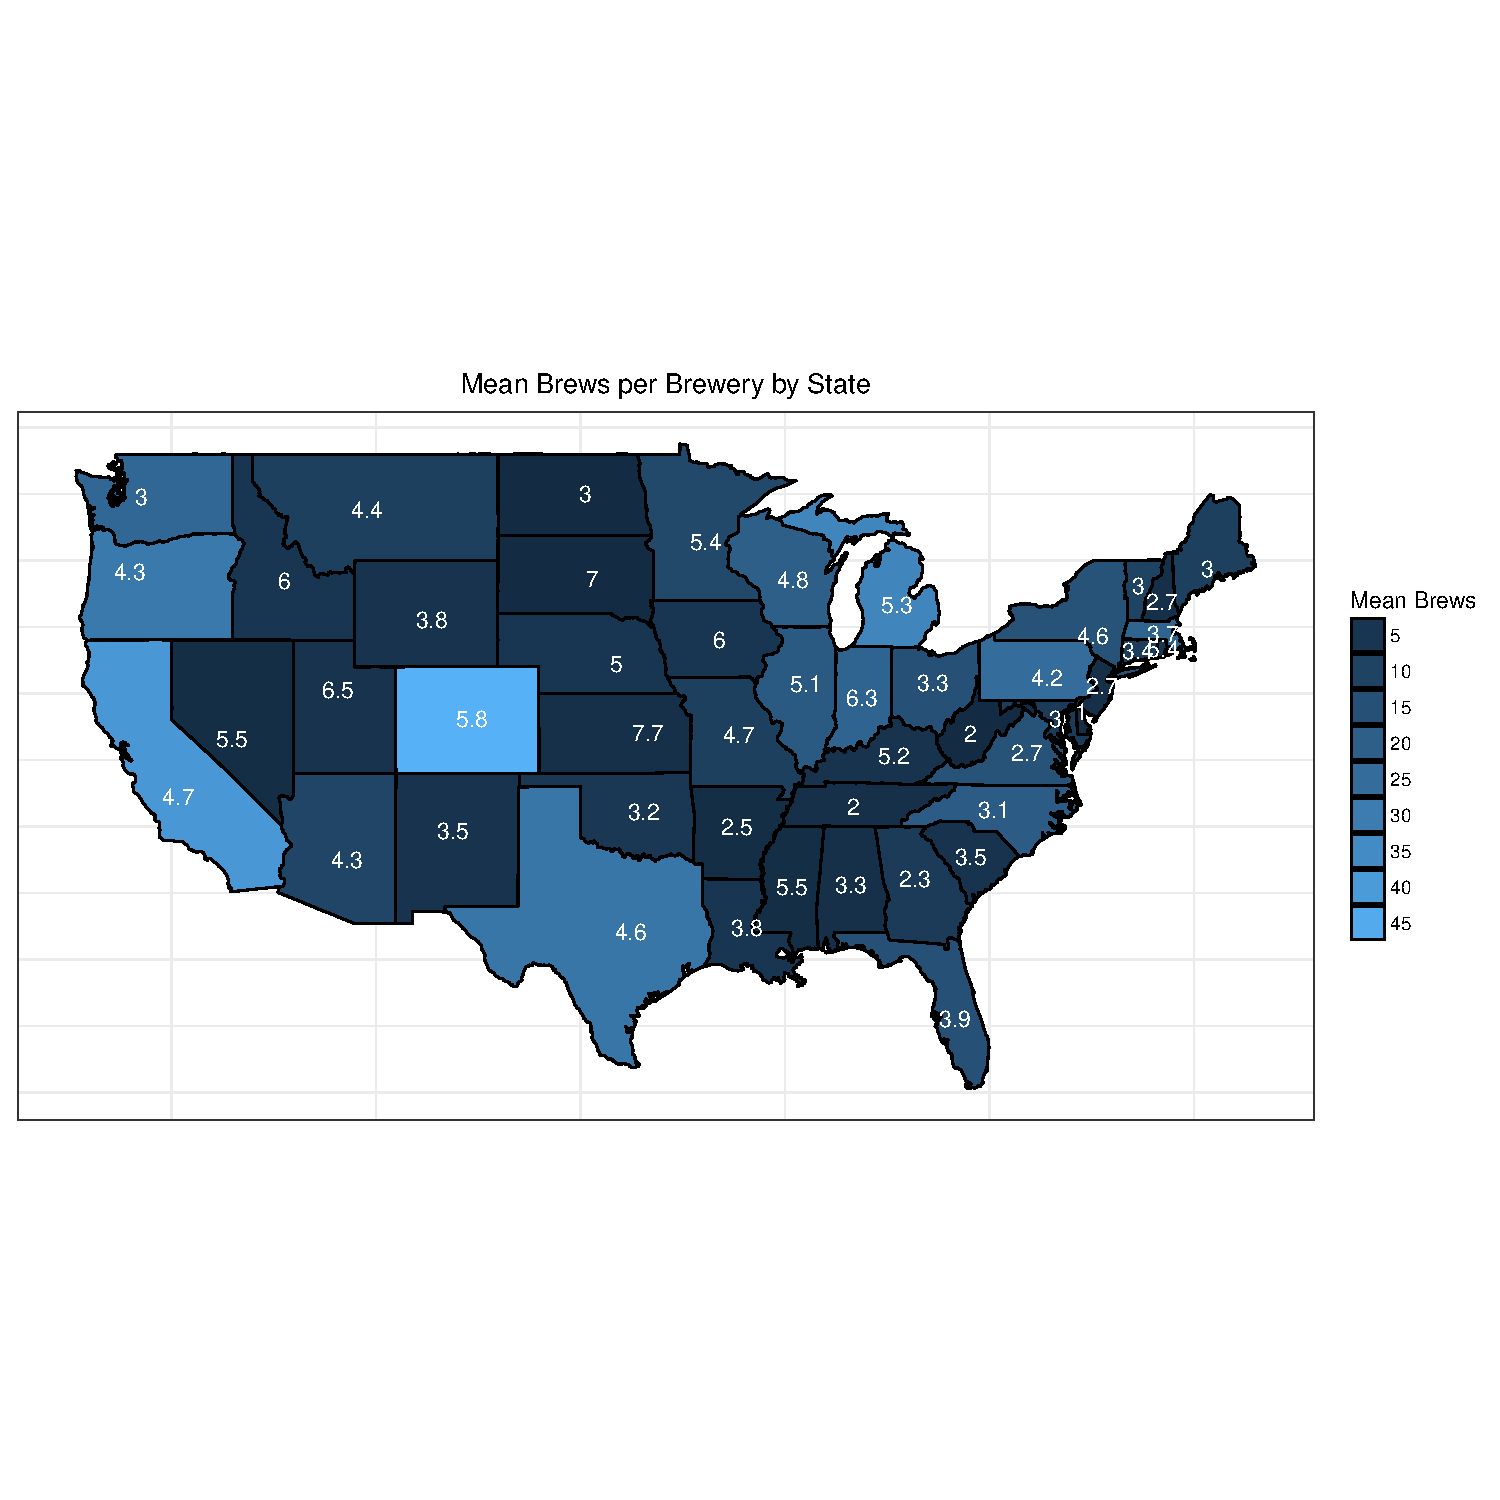
\includegraphics{Analysis_Final_files/figure-latex/unnamed-chunk-16-1} \end{center}

\subsection{Question 3}\label{question-3}

Sometimes data are not available. This analysis is no exception. To
better understand how our analysis could be impacted by missing values
we first have to identify and county them.

These missing values would interfere with our analysis of center for the
numeric variables and frequency of our factor and character variables.
Once the missing values are removed, we can use the clean data to
conduct the descriptive and quantitative analysis.

Below is a count missing values by variable.

\begin{Shaded}
\begin{Highlighting}[]
\CommentTok{# Number of nulls in each column}
\KeywordTok{kable}\NormalTok{(merged_data }\OperatorTok
\StringTok{  }\KeywordTok{select_if}\NormalTok{(}\ControlFlowTok{function}\NormalTok{(x) }\KeywordTok{any}\NormalTok{(}\KeywordTok{is.na}\NormalTok{(x))) }\OperatorTok\StringTok{ }
\StringTok{  }\KeywordTok{summarise_all}\NormalTok{(}\KeywordTok{funs}\NormalTok{(}\KeywordTok{sum}\NormalTok{(}\KeywordTok{is.na}\NormalTok{(.))))}
\NormalTok{)}
\end{Highlighting}
\end{Shaded}

\begin{longtable}[]{@{}rr@{}}
\toprule
abv & ibu\tabularnewline
\midrule
\endhead
62 & 1012\tabularnewline
\bottomrule
\end{longtable}

\subsection{Question 4}\label{question-4}

Computing the median is straightforward. We simply merge all of the
cleaned data by state, and calculate the median ABV and IBU for each
state, which is summarized into a table and plotted as bar charts
recording the median values across each state side by side.

This plot is benificial to the analysis, because it gives insight into
the beer characteristics of the prominent brewing states and the other
states with less than twenty breweries. The prominent brewing states all
share high ABV and IBU values, which brings more evidence to investigate
for the analysis.

Are high ABV and IBU values always a characteristic of highly demanded
beers in the respective market? We will have to produce a plausable
claim and conduct a hypothesis test of that claim after further
investigation.

\begin{Shaded}
\begin{Highlighting}[]
\CommentTok{#TODO: Make bar plot pretty}

\NormalTok{merged_by_state <-}\StringTok{ }\KeywordTok{select}\NormalTok{(merged_data, state, abv, ibu) }\OperatorTok
\StringTok{                   }\KeywordTok{group_by}\NormalTok{(state) }\OperatorTok
\StringTok{                   }\KeywordTok{summarise_all}\NormalTok{(median, }\DataTypeTok{na.rm =} \OtherTok{TRUE}\NormalTok{) }\OperatorTok
\StringTok{                   }\KeywordTok{na.omit}\NormalTok{()}
                    

\NormalTok{merged_by_state}\OperatorTok{$}\NormalTok{state <-}\StringTok{ }\KeywordTok{as.factor}\NormalTok{(merged_by_state}\OperatorTok{$}\NormalTok{state)  }

\CommentTok{#kable(as.data.frame(summarytools::descr(beer_clean)),digits = 2)}


\CommentTok{#TODO: facet by state}

\KeywordTok{ggplot}\NormalTok{(merged_by_state, }
       \KeywordTok{aes}\NormalTok{(}\DataTypeTok{x=}\NormalTok{state, }\DataTypeTok{y=}\NormalTok{abv)) }\OperatorTok{+}
\StringTok{  }\KeywordTok{geom_bar}\NormalTok{(}\DataTypeTok{stat =} \StringTok{"identity"}\NormalTok{,  }
           \DataTypeTok{fill =}\NormalTok{ abv_fill, }
           \DataTypeTok{color =}\NormalTok{ abv_outline, }
           \DataTypeTok{width=}\DecValTok{1}\NormalTok{) }\OperatorTok{+}
\StringTok{  }\KeywordTok{theme}\NormalTok{(}\DataTypeTok{text =} \KeywordTok{element_text}\NormalTok{(}\DataTypeTok{size=}\DecValTok{10}\NormalTok{),}
        \DataTypeTok{axis.text.x =} \KeywordTok{element_text}\NormalTok{(}\DataTypeTok{angle=}\DecValTok{90}\NormalTok{, }\DataTypeTok{hjust=}\DecValTok{0}\NormalTok{, }\DataTypeTok{vjust =}\NormalTok{ .}\DecValTok{3}\NormalTok{))  }\OperatorTok{+}
\StringTok{  }\KeywordTok{theme}\NormalTok{(}\DataTypeTok{legend.position=}\StringTok{"none"}\NormalTok{) }\OperatorTok{+}
\StringTok{  }\KeywordTok{ggtitle}\NormalTok{(}\StringTok{"Median Alcohol Content by State"}\NormalTok{) }\OperatorTok{+}
\StringTok{  }\KeywordTok{xlab}\NormalTok{(}\StringTok{"Alcohol Content (%)"}\NormalTok{) }\OperatorTok{+}
\StringTok{  }\KeywordTok{ylab}\NormalTok{(}\StringTok{"International Bitterness Units (IBU)"}\NormalTok{) }\OperatorTok{+}
\StringTok{  }\KeywordTok{theme}\NormalTok{(}\DataTypeTok{plot.title =} \KeywordTok{element_text}\NormalTok{(}\DataTypeTok{hjust =} \FloatTok{0.5}\NormalTok{))}
\end{Highlighting}
\end{Shaded}

\begin{center}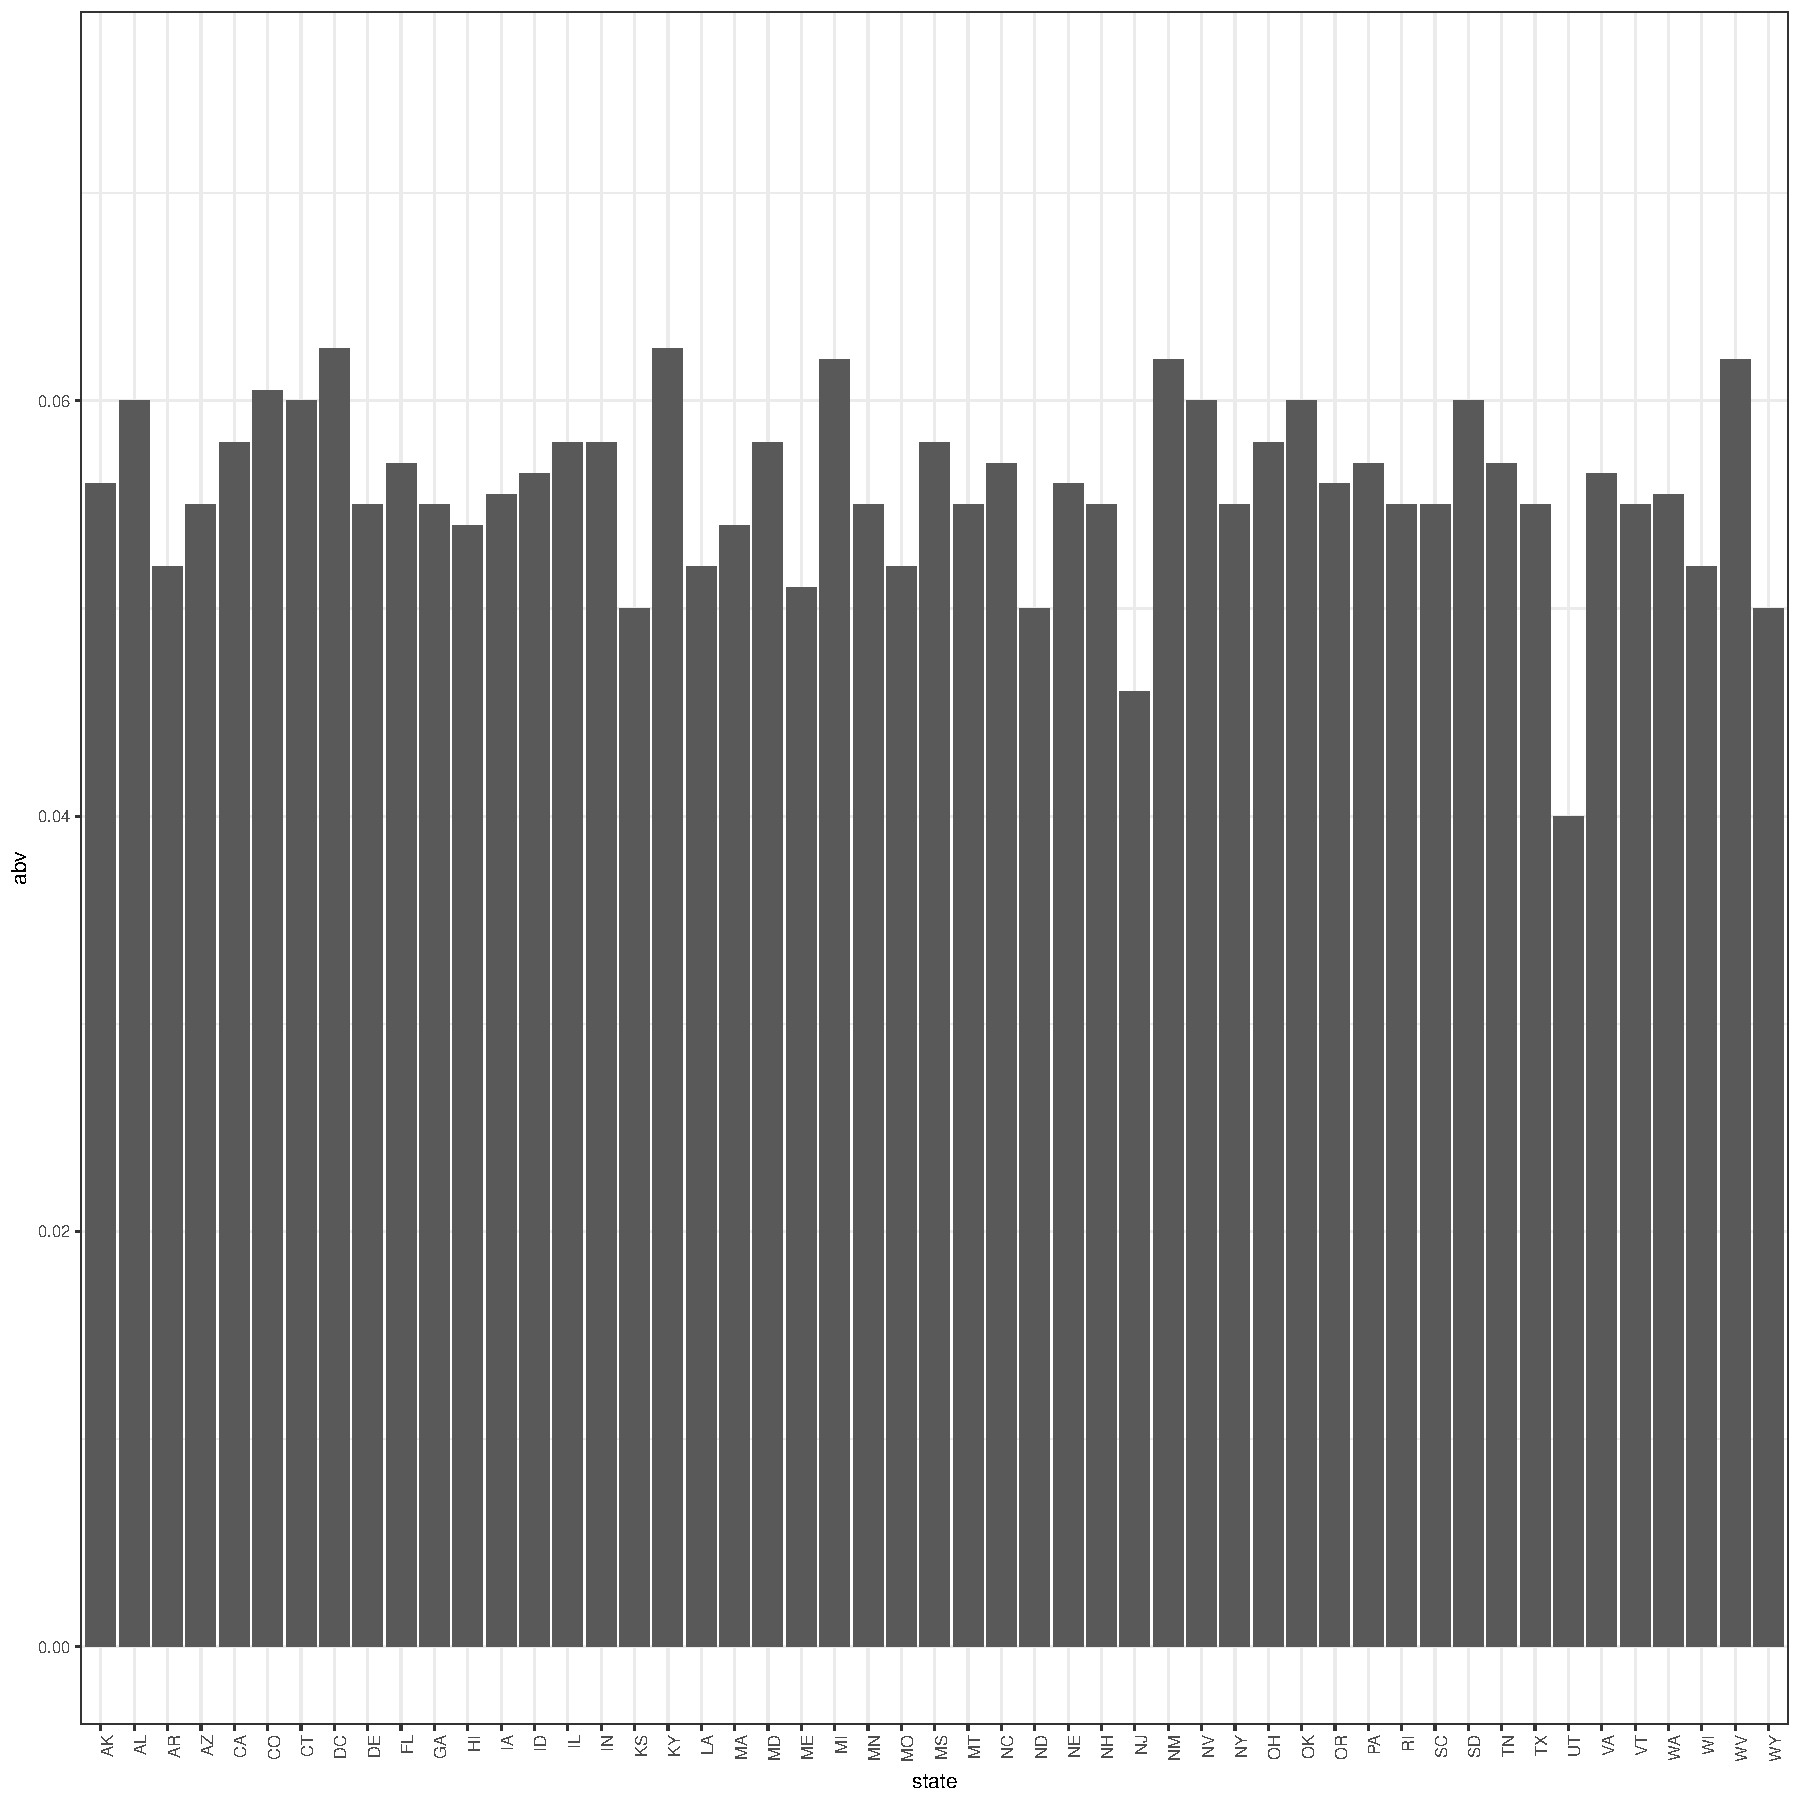
\includegraphics{Analysis_Final_files/figure-latex/unnamed-chunk-18-1} \end{center}

\begin{Shaded}
\begin{Highlighting}[]
\KeywordTok{ggplot}\NormalTok{(merged_by_state, }
       \KeywordTok{aes}\NormalTok{(}\DataTypeTok{x=}\NormalTok{state, }\DataTypeTok{y=}\NormalTok{ibu)) }\OperatorTok{+}
\StringTok{  }\KeywordTok{geom_bar}\NormalTok{(}\DataTypeTok{stat =} \StringTok{"identity"}\NormalTok{,  }
           \DataTypeTok{fill =}\NormalTok{ ibu_fill, }
           \DataTypeTok{color =}\NormalTok{ ibu_outline, }
           \DataTypeTok{width=}\DecValTok{1}\NormalTok{) }\OperatorTok{+}
\StringTok{  }\KeywordTok{theme}\NormalTok{(}\DataTypeTok{text =} \KeywordTok{element_text}\NormalTok{(}\DataTypeTok{size=}\DecValTok{10}\NormalTok{),}
        \DataTypeTok{axis.text.x =} \KeywordTok{element_text}\NormalTok{(}\DataTypeTok{angle=}\DecValTok{90}\NormalTok{, }\DataTypeTok{hjust=}\DecValTok{1}\NormalTok{)) }\OperatorTok{+}
\StringTok{  }\KeywordTok{theme}\NormalTok{(}\DataTypeTok{legend.position=}\StringTok{"none"}\NormalTok{) }\OperatorTok{+}
\StringTok{  }\KeywordTok{ggtitle}\NormalTok{(}\StringTok{"Median Bitterness by State"}\NormalTok{) }\OperatorTok{+}
\StringTok{  }\KeywordTok{xlab}\NormalTok{(}\StringTok{"Alcohol Content (%)"}\NormalTok{) }\OperatorTok{+}
\StringTok{  }\KeywordTok{ylab}\NormalTok{(}\StringTok{"International Bitterness Units (IBU)"}\NormalTok{) }\OperatorTok{+}
\StringTok{  }\KeywordTok{theme}\NormalTok{(}\DataTypeTok{plot.title =} \KeywordTok{element_text}\NormalTok{(}\DataTypeTok{hjust =} \FloatTok{0.5}\NormalTok{))}
\end{Highlighting}
\end{Shaded}

\begin{center}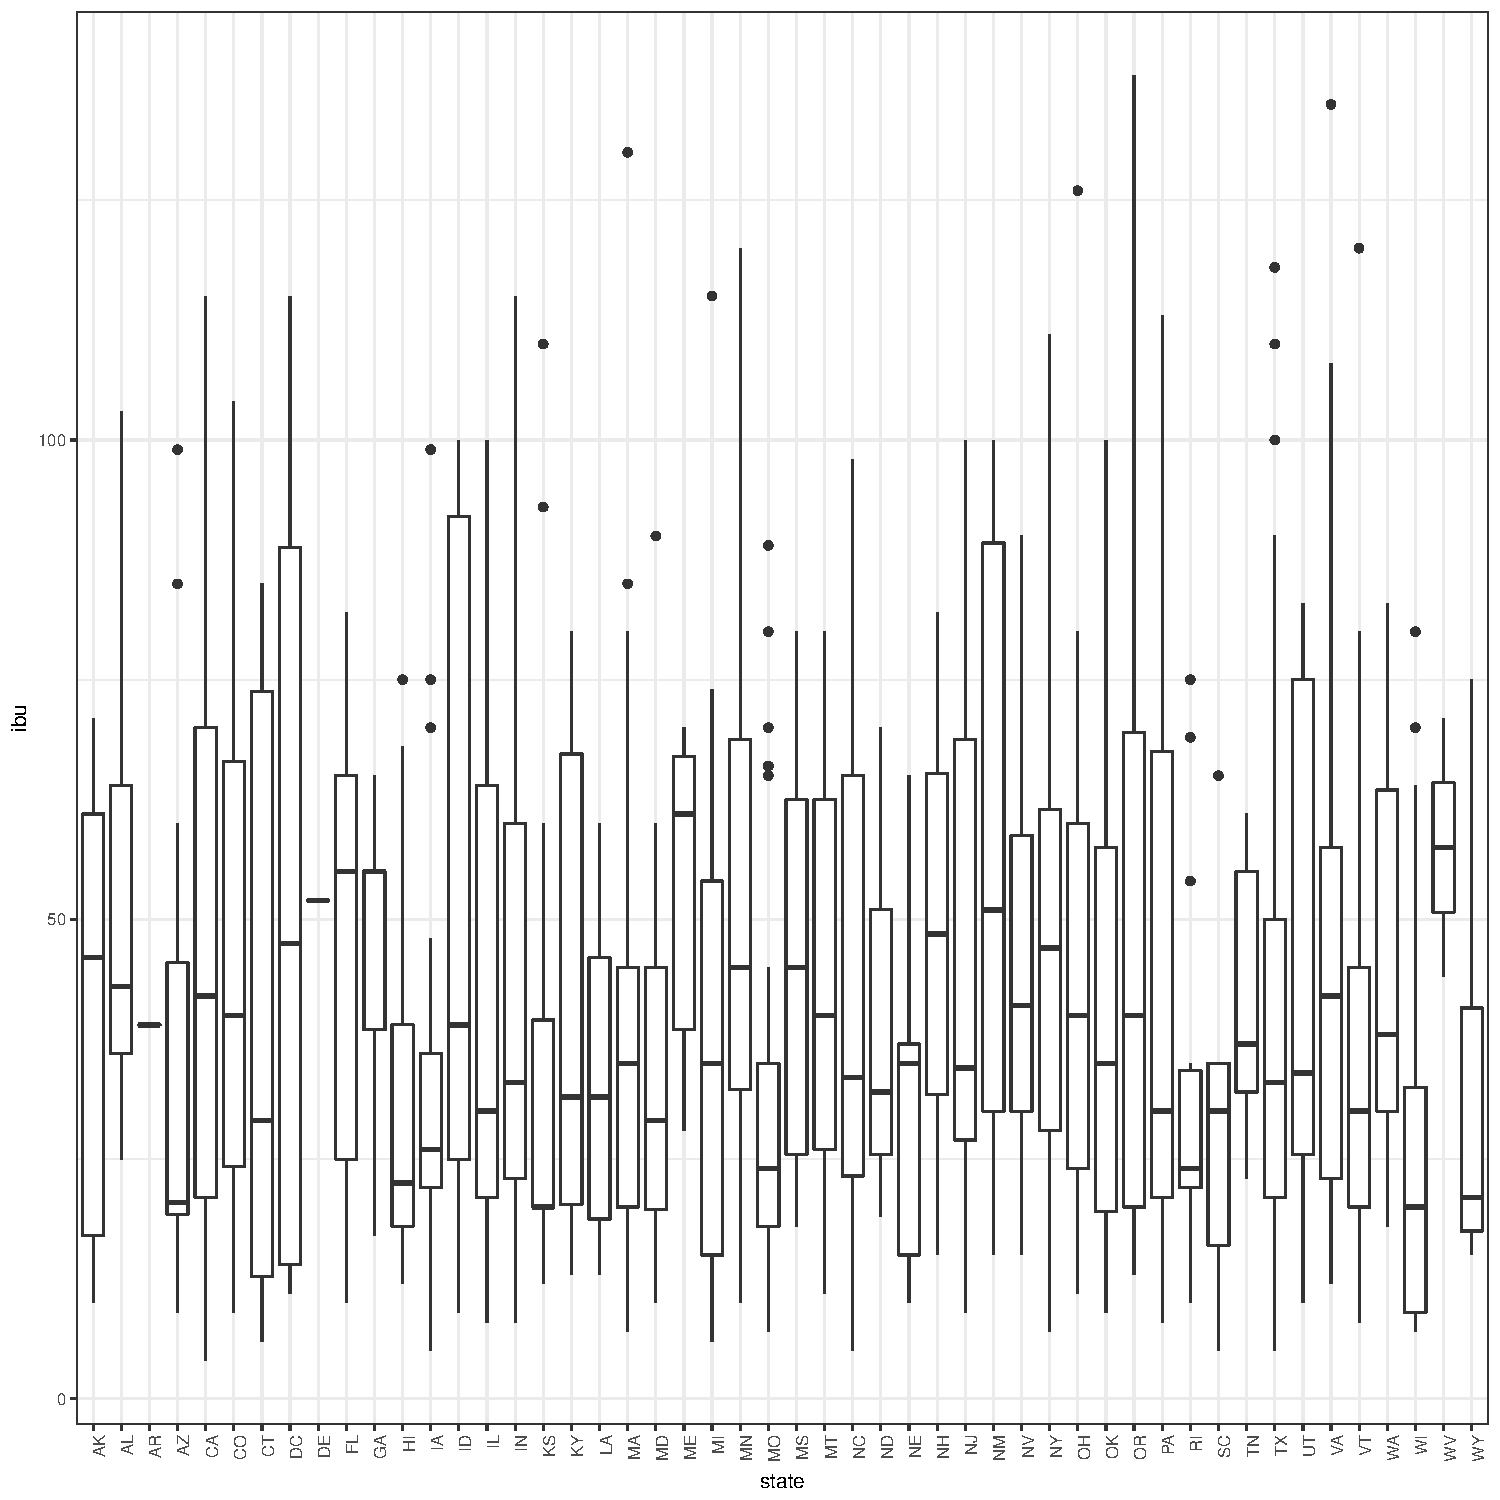
\includegraphics{Analysis_Final_files/figure-latex/unnamed-chunk-18-2} \end{center}

\subsection{Question 5}\label{question-5}

Before you can ``push the limits'' you have to know what the limits are.
We want to determine which state has the most alcoholic beer and which
state has the most bitter beer.

This is relatively simple. We can determine this visually using boxplots
and confirm programmatically by sorting the tables in descending order
based on the values of interest.

The state with the highest ABV value is Colorado with a 0.128 ABV value
for the Lee Hill Series Vol. 5 - Belgian Style Quadrupel Ale beer that
is a Quadrupel (Quad) style of beer brewed by the Upslope Brewing
Company in Boulder, CO.

The state with the highest IBU value is Oregon with a 138 IBU value for
the Bitter Bitch Imperial IPA beer that is a American Double / Imperial
IPA style of beer brewed by the Astoria Brewing Company in Astoria, OR.

The states with the highest ABV and IBU values are found to be comprised
of a majority of the prominent brewing states including the folling
values State(maxABV, maxIBU):

Colorado(.128, 104), California(.099, 115), Michigan(.099, 115),
Oregon(.082, 138), Texas(.099, 118), Pennsylvania(.099, 113),
Massachusetts(.099, 130), Washington(.084, 83), Indiana(.120, 115),
Wisconsin(.099, 80).

\begin{Shaded}
\begin{Highlighting}[]
\KeywordTok{ggplot}\NormalTok{((merged_data }\OperatorTok\StringTok{ }\KeywordTok{na.omit}\NormalTok{(abv)), }
       \KeywordTok{aes}\NormalTok{(}\DataTypeTok{x=}\NormalTok{state , }\DataTypeTok{y=}\NormalTok{abv)) }\OperatorTok{+}\StringTok{  }\CommentTok{#TODO: Move to Appendix}
\StringTok{  }\KeywordTok{geom_boxplot}\NormalTok{() }\OperatorTok{+}
\StringTok{  }\CommentTok{#ylim(0, .075) +}
\StringTok{  }\KeywordTok{theme}\NormalTok{(}\DataTypeTok{text =} \KeywordTok{element_text}\NormalTok{(}\DataTypeTok{size=}\DecValTok{10}\NormalTok{),}
        \DataTypeTok{axis.text.x =} \KeywordTok{element_text}\NormalTok{(}\DataTypeTok{angle=}\DecValTok{90}\NormalTok{, }\DataTypeTok{hjust=}\DecValTok{1}\NormalTok{)) }
\end{Highlighting}
\end{Shaded}

\begin{center}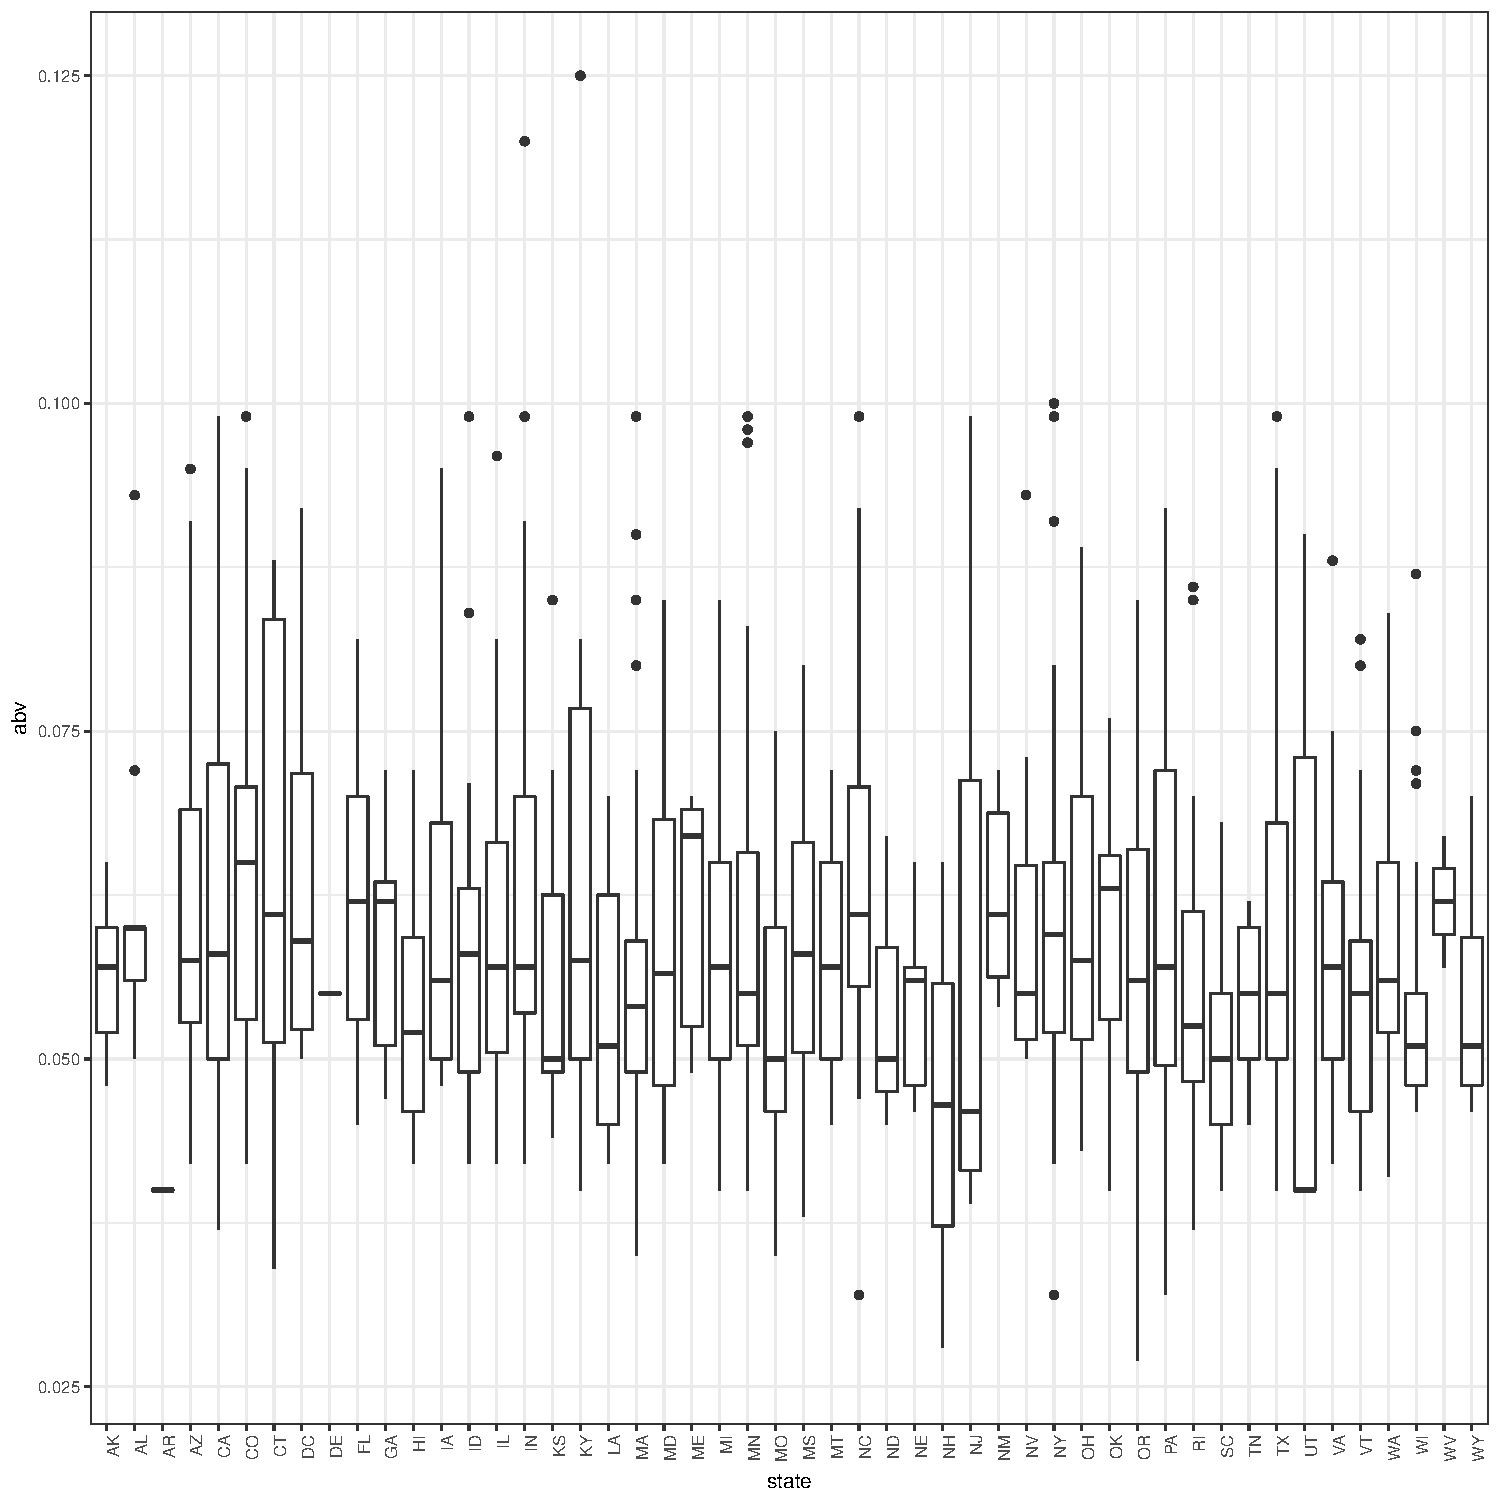
\includegraphics{Analysis_Final_files/figure-latex/unnamed-chunk-19-1} \end{center}

\begin{Shaded}
\begin{Highlighting}[]
\KeywordTok{ggplot}\NormalTok{((merged_data }\OperatorTok\StringTok{ }\KeywordTok{na.omit}\NormalTok{(ibu)), }
       \KeywordTok{aes}\NormalTok{(}\DataTypeTok{x=}\NormalTok{state , }\DataTypeTok{y=}\NormalTok{ibu)) }\OperatorTok{+}\StringTok{  }\CommentTok{#TODO: Move to Appendix}
\StringTok{  }\KeywordTok{geom_boxplot}\NormalTok{() }\OperatorTok{+}
\StringTok{  }\CommentTok{#ylim(0, .075) +}
\StringTok{  }\KeywordTok{theme}\NormalTok{(}\DataTypeTok{text =} \KeywordTok{element_text}\NormalTok{(}\DataTypeTok{size=}\DecValTok{10}\NormalTok{),}
        \DataTypeTok{axis.text.x =} \KeywordTok{element_text}\NormalTok{(}\DataTypeTok{angle=}\DecValTok{90}\NormalTok{, }\DataTypeTok{hjust=}\DecValTok{1}\NormalTok{)) }
\end{Highlighting}
\end{Shaded}

\begin{center}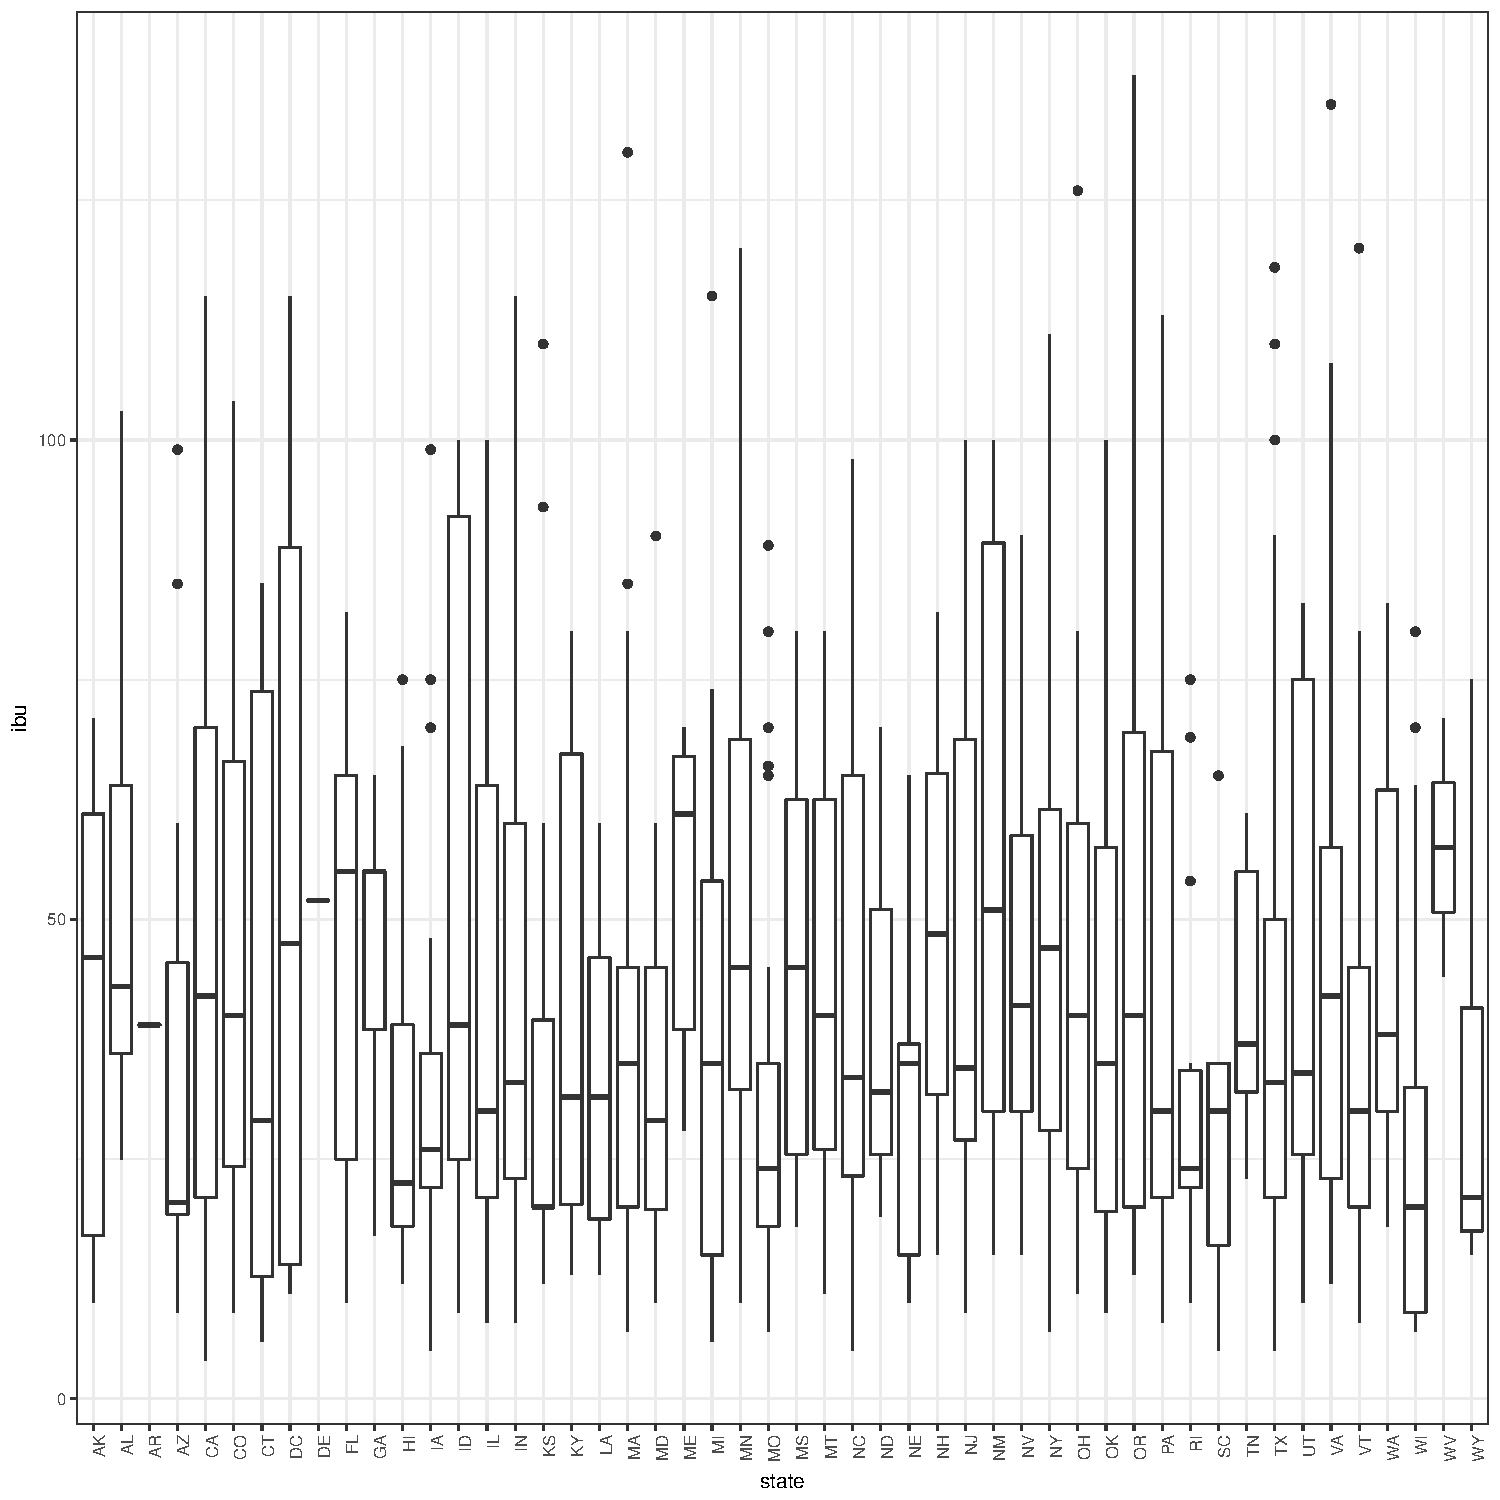
\includegraphics{Analysis_Final_files/figure-latex/unnamed-chunk-19-2} \end{center}

\begin{Shaded}
\begin{Highlighting}[]
\NormalTok{max_abv <-}\StringTok{  }\NormalTok{(}\KeywordTok{select}\NormalTok{(merged_data, state, abv) }\OperatorTok
\StringTok{                   }\KeywordTok{group_by}\NormalTok{(state) }\OperatorTok
\StringTok{                   }\KeywordTok{arrange}\NormalTok{(}\KeywordTok{desc}\NormalTok{(abv))  }\OperatorTok\StringTok{ }\CommentTok{#sort by ABV}
\StringTok{                   }\KeywordTok{filter}\NormalTok{(}\KeywordTok{row_number}\NormalTok{() }\OperatorTok{==}\StringTok{ }\DecValTok{1}\NormalTok{))[}\DecValTok{1}\NormalTok{,] }\CommentTok{#get first row}
          
\NormalTok{max_abv}
\end{Highlighting}
\end{Shaded}

\section{A tibble: 1 x 2}\label{a-tibble-1-x-2}

\section{Groups: state {[}1{]}}\label{groups-state-1}

state abv 1 CO 0.128

\begin{Shaded}
\begin{Highlighting}[]
\NormalTok{max_ibu <-}\StringTok{  }\NormalTok{(}\KeywordTok{select}\NormalTok{(merged_data, state, ibu) }\OperatorTok
\StringTok{                   }\KeywordTok{group_by}\NormalTok{(state) }\OperatorTok
\StringTok{                   }\KeywordTok{arrange}\NormalTok{(}\KeywordTok{desc}\NormalTok{(ibu))  }\OperatorTok\StringTok{ }\CommentTok{#sort by ABV}
\StringTok{                   }\KeywordTok{filter}\NormalTok{(}\KeywordTok{row_number}\NormalTok{() }\OperatorTok{==}\StringTok{ }\DecValTok{1}\NormalTok{))[}\DecValTok{1}\NormalTok{,] }\CommentTok{#get first row}
          
\NormalTok{max_ibu}
\end{Highlighting}
\end{Shaded}

\section{A tibble: 1 x 2}\label{a-tibble-1-x-2-1}

\section{Groups: state {[}1{]}}\label{groups-state-1-1}

state ibu 1 OR 138

\subsection{Question 6}\label{question-6}

The amount of alcohol by volume ABV is a good representation of the beer
market, where consumer demand is infered from the geographical spread
and number of breweries produce a certain style of beer. The certain
style of a beer is controlled in-part by the ABV content. From the ABV
five number summary we can better describe the use of the ABV variable
as a controlling factor in the consumer market of beer.

The minimum ABV value of 0.001 is represented only one style of beer
-Low Alcohol Beer produced by 1 brewery in CA:1. From these data we can
infer the lack of consumer demand by the geographical spread of the
style and by the lack of 0.001 ABV variability.

The first quartile(Q1) is represented by beers with a 0.050 ABV value
represented by the -American -IPA and -Ale styles of beer that ranges
from 5-100 in IBU. There are 38 different styles of beers with this ABV,
that are produced by 141 different breweries in 46 different states
AK:3, AL:1, AR:1, AZ:3, CA:10, CO:12, CT:3, DC:1, FL:5, GA:1, HI:1,
IA:3, ID:2, IL:4, IN:3, KS:2, KY:1, LA:3, MA:4, MD:2, ME:2, MI:8, MN:3,
MO:3, MS:1, MT:3, NC:4, ND:1, NE:1, NH:1, NJ:1, NV:1, NY:1, OH:6, Ok:1,
OR:8, PA:5, RI:1, SC:1, TN:1, TX:5, UT:2, VA:2, WA:2, WI:7, WY:2. The
use of a 0.050 ABV for a beer will allow for a large amount of variation
with respect to the IBU of a beer style. The use of an ABV of 0.050 with
any IBU between 5-100 will likely be a higly demanded beer by the
consumer market.

The median ABV value of 0.056 represents the -American Ale and -Pale Ale
styles of beer that ranges from 4-70 in IBU. There are 21 different
styles of beers with this ABV, that are produced by 49 different
breweries in 25 different states AK:1, AL:1, CA:5, CO:6, FL:1, IA:1,
ID:1, IL:2, IN:2, KS:1, MA:3, MI:4, MN:2, MO:1, MT:1, NC:1, NE:1, NH:1,
NY:1, OR:1, PA:4, TX:3, VA:2, WA:1, WI:2.

The third quartile(Q3) is represented by beers with a 0.067 ABV value
represented by the -IPA and -Ale styles of beer that ranges from 33-85
in IBU. There are 10 different styles of beers with this ABV, that are
produced by 22 different breweries in 15 different states AZ:1, CA:2,
CO:3, MA:1, ME:1, MI:4, MN:2, NC:1, ND:1, NY:1, OH:1, OR:4, PA:1, WA:1,
WV:1.

The maximum ABV value of 0.128 is represented only one style of beer
-Quadrupel (Quad) that is produce by 3 breweries from 3 different states
CO:1, IN:1, MI:1, and we can infer the demand of the consumer as a
moderate demand by the breweries producing these beer being spread out
geographically across the nation even though the style variability is
very-low for the 0.128 ABV.

Summarizing the statistics for ABV can be accomplished in a signle
command.

\begin{Shaded}
\begin{Highlighting}[]
\CommentTok{#summaryize ABV}


\NormalTok{abv_stats <-}\StringTok{ }\KeywordTok{select}\NormalTok{(merged_data, abv) }\OperatorTok\StringTok{ }\CommentTok{#select columns}
\StringTok{                   }\KeywordTok{na.omit}\NormalTok{() }\OperatorTok\StringTok{ }\CommentTok{# omit nulls}
\StringTok{                   }\NormalTok{dplyr}\OperatorTok{::}\KeywordTok{summarize_all}\NormalTok{(}\KeywordTok{funs}\NormalTok{(}\DataTypeTok{count=}\KeywordTok{n}\NormalTok{(), }\KeywordTok{min}\NormalTok{(abv), }\KeywordTok{max}\NormalTok{(abv), }\KeywordTok{mean}\NormalTok{(abv), }\KeywordTok{median}\NormalTok{(abv), }\KeywordTok{sd}\NormalTok{(abv)))}

\NormalTok{ibu_stats <-}\StringTok{ }\KeywordTok{select}\NormalTok{(merged_data, ibu) }\OperatorTok\StringTok{ }\CommentTok{#select columns}
\StringTok{                   }\KeywordTok{na.omit}\NormalTok{() }\OperatorTok\StringTok{ }\CommentTok{# omit nulls}
\StringTok{                   }\NormalTok{dplyr}\OperatorTok{::}\KeywordTok{summarize_all}\NormalTok{(}\KeywordTok{funs}\NormalTok{(}\DataTypeTok{count=}\KeywordTok{n}\NormalTok{(), }\KeywordTok{min}\NormalTok{(ibu), }\KeywordTok{max}\NormalTok{(ibu), }\KeywordTok{mean}\NormalTok{(ibu), }\KeywordTok{median}\NormalTok{(ibu), }\KeywordTok{sd}\NormalTok{(ibu)))}


\KeywordTok{kable}\NormalTok{(abv_stats)}
\end{Highlighting}
\end{Shaded}

\begin{longtable}[]{@{}rrrrrr@{}}
\toprule
count & min & max & mean & median & sd\tabularnewline
\midrule
\endhead
2363 & 0.001 & 0.128 & 0.0597647 & 0.056 & 0.0135242\tabularnewline
\bottomrule
\end{longtable}

\subsection{Question 7}\label{question-7}

To determine the relationship between ABV and IBU it's helpful to see
all values for both variables at the same time. This is most easily
accomplished using a scatterplot.

Linear regression was used to model the relationship between ABV and IBU
from a sample of cleaned data that was created in the previous questions
above.

The equation:

\begin{verbatim}
   y-intercept = IBU - slope * ABV       
\end{verbatim}

was used to plot thw linear model for the ABV and IBU data in this
study.

With ABV on the x-axis and IBU on the y-axis, we start to see that there
is a positive linear correlation between the ABV and IBU values, with
R-squared = 0.44593.

R-squared is a statistical measure of how close the data are to the
fitted regression line. It is also known as the coefficient of
determination, and the definition of R-squared is fairly
straight-forward; it is the percentage of the response variable
variation that is explained by the linear model.

Since the creation, consumption, and distribution of beer by methods of
breweries is a human behavior, it is very important to note that it is
common for studies to measure R-squared values less than 0.50. The
reason is , that human behavior is harder to predict with linear models.

The outcome of our study measured an R-squared value of 0.44593 which is
an awesome fit, and much better than we expected for this study to
produce, since the study is based on the human behavior of beer
consumption with respect to the variation of ABV and IBU accross the
United States of America.

Adding a trendline allows us to determine a formula that specifies this
correlation. The regression is plotted and the results of the Spearman's
Rank Correlation Test are in the following figures.

\subsubsection{Spearman's Rank Correlation Results for
rho}\label{spearmans-rank-correlation-results-for-rho}

\begin{Shaded}
\begin{Highlighting}[]
\NormalTok{data}\OperatorTok{:}\StringTok{  }\NormalTok{styles}\OperatorTok{$}\NormalTok{ibu and styles}\OperatorTok{$}\NormalTok{abv}
\NormalTok{S =}\StringTok{ }\DecValTok{153570000}\NormalTok{, p}\OperatorTok{-}\NormalTok{value }\OperatorTok{<}\StringTok{ }\FloatTok{2.2e-16}
\NormalTok{alternative hypothesis}\OperatorTok{:}\StringTok{ }\NormalTok{true rho is not equal to }\DecValTok{0}
\NormalTok{sample estimates}\OperatorTok{:}
\NormalTok{rho }
\FloatTok{0.6677798} 

\NormalTok{[}\DecValTok{1}\NormalTok{] }\FloatTok{0.4459299}
\end{Highlighting}
\end{Shaded}

\begin{Shaded}
\begin{Highlighting}[]
\CommentTok{#A distinct list of beer styles, as classified by a unique style Name, IBU, ABV, and Ounces values.}

\NormalTok{styles <-}\StringTok{ }\NormalTok{beer_clean }\OperatorTok\StringTok{ }
\StringTok{              }\KeywordTok{distinct}\NormalTok{(beer_id, style, ibu, abv, ounces) }\OperatorTok\StringTok{ }
\StringTok{              }\KeywordTok{arrange}\NormalTok{(style) }\OperatorTok\StringTok{ }
\StringTok{              }\KeywordTok{na.omit}\NormalTok{(ibu, abv)}
\end{Highlighting}
\end{Shaded}

\begin{itemize}
\tightlist
\item
  Plot ABV v. IBU
\end{itemize}

\begin{Shaded}
\begin{Highlighting}[]
\KeywordTok{ggplot}\NormalTok{(styles, }\KeywordTok{aes}\NormalTok{(}\DataTypeTok{x=}\NormalTok{abv, }\DataTypeTok{y=}\NormalTok{ibu)) }\OperatorTok{+}
\StringTok{  }\KeywordTok{geom_point}\NormalTok{(}\DataTypeTok{color =}\NormalTok{ misc_cool,}
             \DataTypeTok{size =} \DecValTok{3}\NormalTok{) }\OperatorTok{+}
\StringTok{  }\KeywordTok{theme}\NormalTok{(}\DataTypeTok{legend.position=}\StringTok{"none"}\NormalTok{) }\OperatorTok{+}
\StringTok{  }\KeywordTok{ggtitle}\NormalTok{(}\StringTok{"Alcohol Content v Bitterness"}\NormalTok{) }\OperatorTok{+}
\StringTok{  }\KeywordTok{xlab}\NormalTok{(}\StringTok{"Alcohol Content (%)"}\NormalTok{) }\OperatorTok{+}
\StringTok{  }\KeywordTok{ylab}\NormalTok{(}\StringTok{"International Bitterness Units (IBU)"}\NormalTok{) }\OperatorTok{+}
\StringTok{  }\KeywordTok{theme}\NormalTok{(}\DataTypeTok{plot.title =} \KeywordTok{element_text}\NormalTok{(}\DataTypeTok{hjust =} \FloatTok{0.5}\NormalTok{))}
\end{Highlighting}
\end{Shaded}

\begin{center}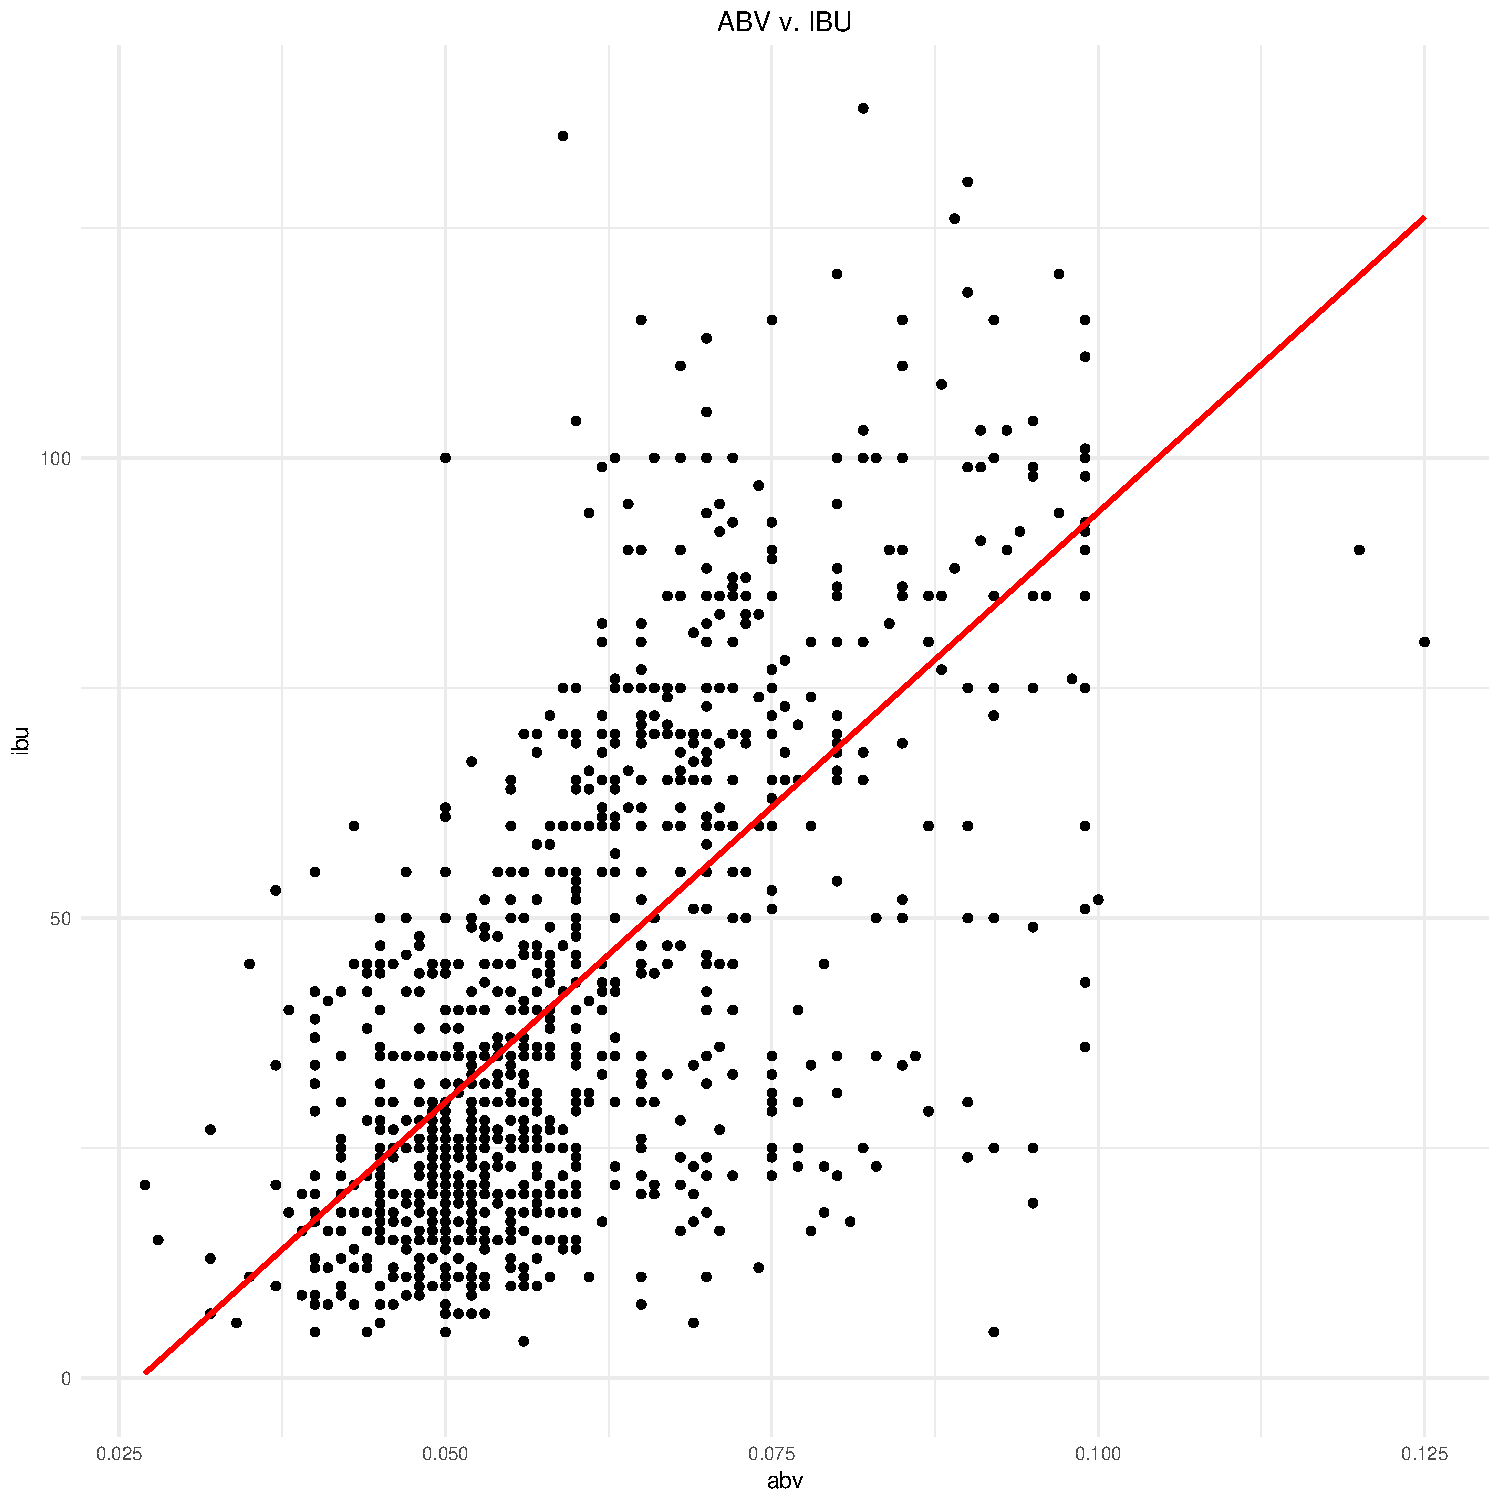
\includegraphics{Analysis_Final_files/figure-latex/unnamed-chunk-22-1} \end{center}

\subsubsection{Analysis of ABV and IBU}\label{analysis-of-abv-and-ibu}

\begin{verbatim}
+ More info on Spearman test: https://statistics.laerd.com/statistical-guides/spearmans-rank-order-correlation-statistical-guide.php
\end{verbatim}

\begin{itemize}
\item
  Problem: We wish to test if there is a monotonic association between
  the alochol by volume (ABV) and international bitterness unit (IBU)
  rating of beers selected from domestic craft breweries.
\item
  Hypotheses:

  \begin{itemize}
  \tightlist
  \item
    H\textsubscript{o}: \(\rho= 0\)
  \item
    H\textsubscript{A}: \(\rho\neq 0\)
  \end{itemize}
\end{itemize}

\begin{itemize}
\tightlist
\item
  Assumptions:

  \begin{itemize}
  \tightlist
  \item
    Continuity of \url{data:/cmark}
  \item
    Paired observations: \cmark
  \item
    Data has linear relationship: \cmark 
  \item
    No significant outliers: \xmark
  \item
    Normality: \xmark
  \end{itemize}
\end{itemize}

\begin{Shaded}
\begin{Highlighting}[]
\CommentTok{#Scatter plot of ABV v IBU}
\KeywordTok{ggplot}\NormalTok{(styles, }\KeywordTok{aes}\NormalTok{(}\DataTypeTok{x=}\NormalTok{abv, }\DataTypeTok{y=}\NormalTok{ibu)) }\OperatorTok{+}
\StringTok{  }\KeywordTok{geom_point}\NormalTok{(}\DataTypeTok{color =}\NormalTok{ misc_cool,}
             \DataTypeTok{size =} \DecValTok{3}\NormalTok{) }\OperatorTok{+}
\StringTok{  }\KeywordTok{geom_smooth}\NormalTok{(}\DataTypeTok{method =} \StringTok{"lm"}\NormalTok{, }
              \DataTypeTok{se =} \OtherTok{FALSE}\NormalTok{, }
              \DataTypeTok{color=}\NormalTok{misc_warm) }\OperatorTok{+}
\StringTok{  }\KeywordTok{theme}\NormalTok{(}\DataTypeTok{legend.position=}\StringTok{"none"}\NormalTok{) }\OperatorTok{+}
\StringTok{  }\KeywordTok{ggtitle}\NormalTok{(}\StringTok{"Alcohol Content v Bitterness"}\NormalTok{) }\OperatorTok{+}
\StringTok{  }\KeywordTok{xlab}\NormalTok{(}\StringTok{"Alcohol Content (%)"}\NormalTok{) }\OperatorTok{+}
\StringTok{  }\KeywordTok{ylab}\NormalTok{(}\StringTok{"International Bitterness Units (IBU)"}\NormalTok{) }\OperatorTok{+}
\StringTok{  }\KeywordTok{theme}\NormalTok{(}\DataTypeTok{plot.title =} \KeywordTok{element_text}\NormalTok{(}\DataTypeTok{hjust =} \FloatTok{0.5}\NormalTok{))}
\end{Highlighting}
\end{Shaded}

\begin{center}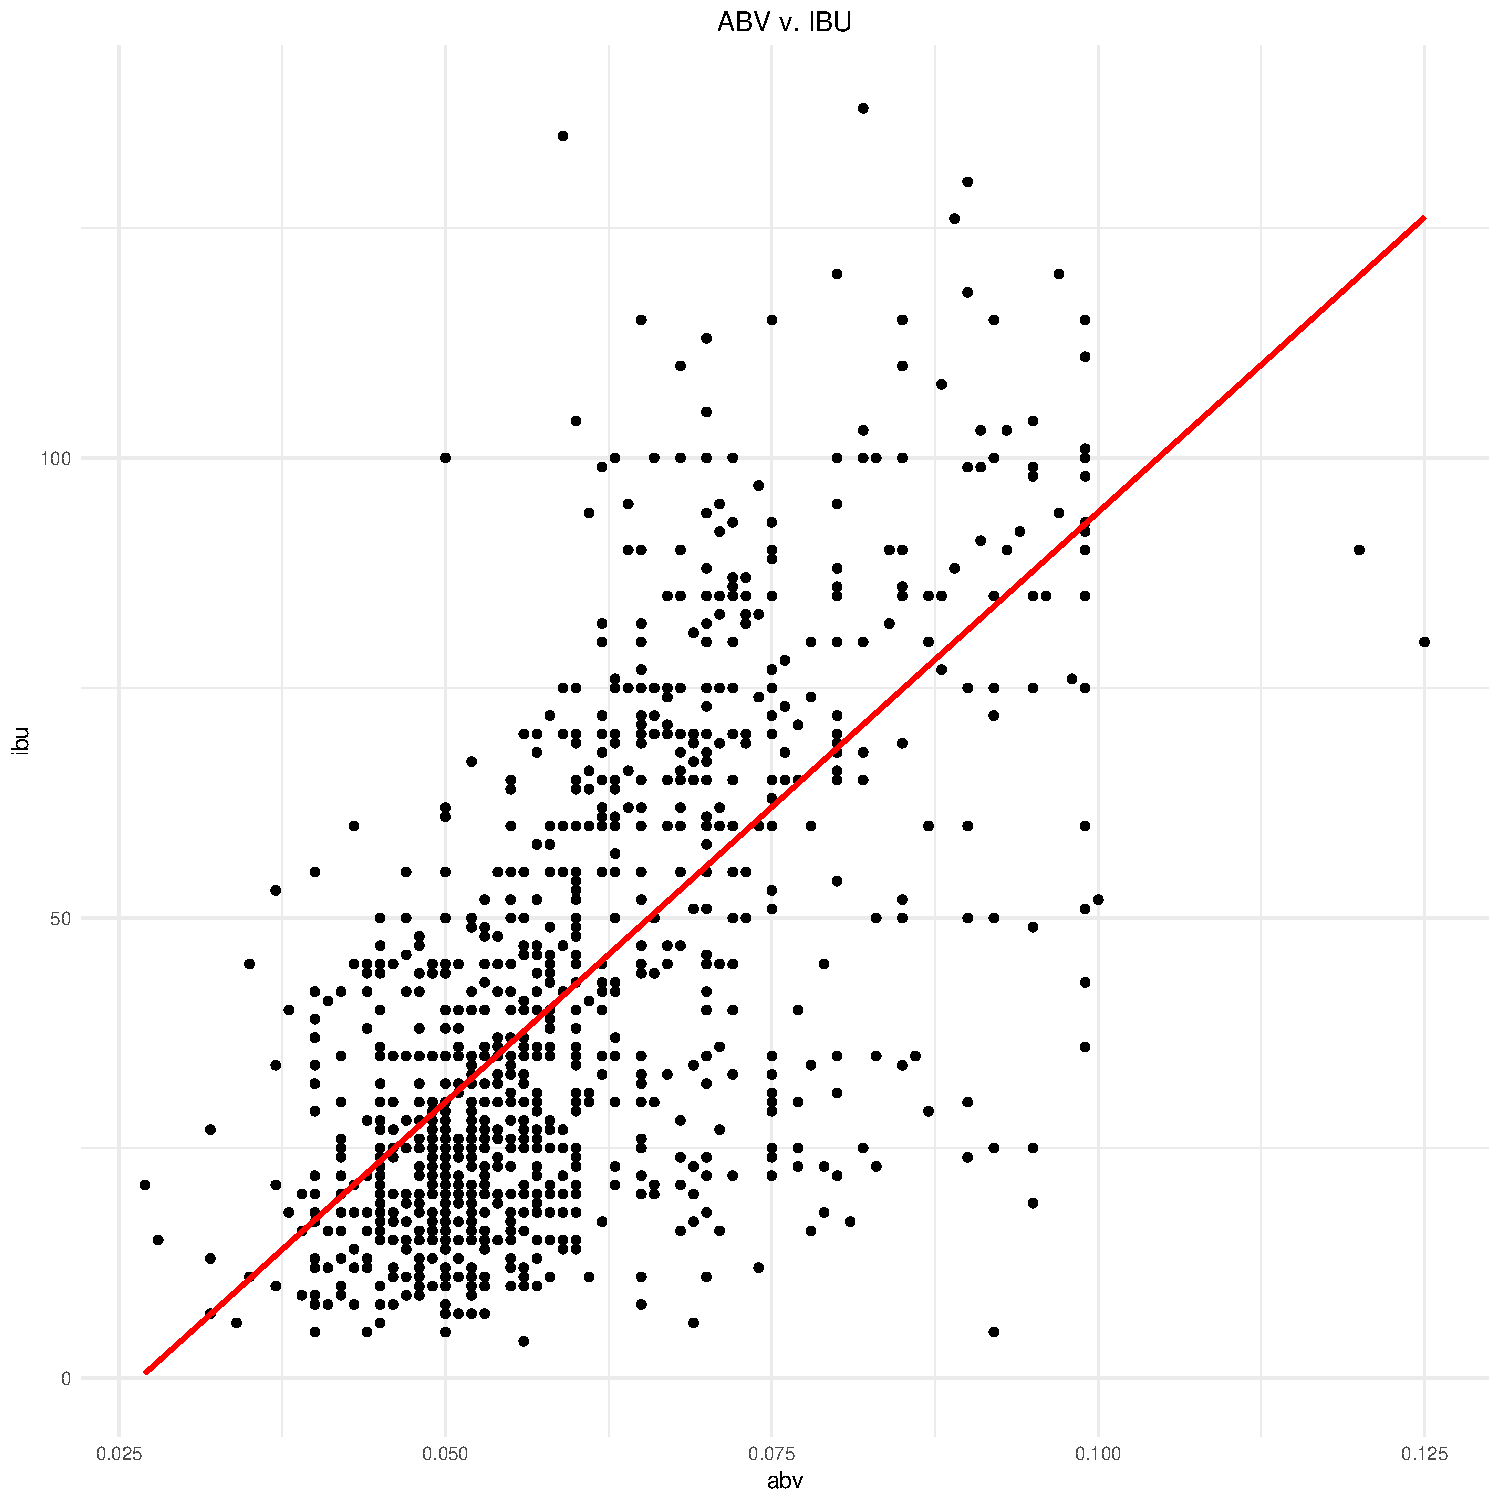
\includegraphics{Analysis_Final_files/figure-latex/unnamed-chunk-23-1} \end{center}

\paragraph{QQ-Plot - Check for
Normality}\label{qq-plot---check-for-normality}

\begin{Shaded}
\begin{Highlighting}[]
\CommentTok{# QQ Plots of IBU and ABV}


\CommentTok{#calulate line fit}
\NormalTok{y <-}\StringTok{ }\KeywordTok{quantile}\NormalTok{((styles}\OperatorTok{$}\NormalTok{ibu }\OperatorTok\StringTok{ }\KeywordTok{na.omit}\NormalTok{()), }\KeywordTok{c}\NormalTok{(}\FloatTok{0.25}\NormalTok{, }\FloatTok{0.75}\NormalTok{))}
\NormalTok{x <-}\StringTok{ }\KeywordTok{qnorm}\NormalTok{(}\KeywordTok{c}\NormalTok{(}\FloatTok{0.25}\NormalTok{, }\FloatTok{0.75}\NormalTok{))}
\NormalTok{slope <-}\StringTok{ }\KeywordTok{diff}\NormalTok{(y)}\OperatorTok{/}\KeywordTok{diff}\NormalTok{(x)}
\NormalTok{y_int <-}\StringTok{ }\NormalTok{y[}\DecValTok{1}\NormalTok{] }\OperatorTok{-}\StringTok{ }\NormalTok{slope }\OperatorTok{*}\StringTok{ }\NormalTok{x[}\DecValTok{1}\NormalTok{]}

\NormalTok{qq_ibu <-}\StringTok{ }\KeywordTok{ggplot}\NormalTok{(styles, }\KeywordTok{aes}\NormalTok{(}\DataTypeTok{sample =}\NormalTok{ styles}\OperatorTok{$}\NormalTok{ibu)) }\OperatorTok{+}\StringTok{ }
\StringTok{              }\KeywordTok{geom_qq}\NormalTok{(}\DataTypeTok{shape =} \DecValTok{16}\NormalTok{, }\DataTypeTok{size =} \DecValTok{2}\NormalTok{, }\DataTypeTok{alpha =} \FloatTok{0.5}\NormalTok{) }\OperatorTok{+}
\StringTok{              }\KeywordTok{geom_abline}\NormalTok{(}\DataTypeTok{slope =}\NormalTok{ slope, }\DataTypeTok{intercept =}\NormalTok{ y_int, }\DataTypeTok{colour =}\StringTok{'red'}\NormalTok{, }\DataTypeTok{size =} \DecValTok{1}\NormalTok{) }\OperatorTok{+}
\StringTok{              }\KeywordTok{ggtitle}\NormalTok{(}\StringTok{"QQ-Plot of IBU"}\NormalTok{) }\OperatorTok{+}
\StringTok{              }\KeywordTok{theme_bw}\NormalTok{()  }\OperatorTok{+}
\StringTok{              }\KeywordTok{theme}\NormalTok{(}\DataTypeTok{plot.title =} \KeywordTok{element_text}\NormalTok{(}\DataTypeTok{hjust =} \FloatTok{0.5}\NormalTok{))}


\CommentTok{#calulate line fit}
\NormalTok{y <-}\StringTok{ }\KeywordTok{quantile}\NormalTok{((styles}\OperatorTok{$}\NormalTok{abv }\OperatorTok\StringTok{ }\KeywordTok{na.omit}\NormalTok{()), }\KeywordTok{c}\NormalTok{(}\FloatTok{0.25}\NormalTok{, }\FloatTok{0.75}\NormalTok{))}
\NormalTok{x <-}\StringTok{ }\KeywordTok{qnorm}\NormalTok{(}\KeywordTok{c}\NormalTok{(}\FloatTok{0.25}\NormalTok{, }\FloatTok{0.75}\NormalTok{))}
\NormalTok{slope <-}\StringTok{ }\KeywordTok{diff}\NormalTok{(y)}\OperatorTok{/}\KeywordTok{diff}\NormalTok{(x)}
\NormalTok{y_int <-}\StringTok{ }\NormalTok{y[}\DecValTok{1}\NormalTok{] }\OperatorTok{-}\StringTok{ }\NormalTok{slope }\OperatorTok{*}\StringTok{ }\NormalTok{x[}\DecValTok{1}\NormalTok{]  }

\NormalTok{qq_abv <-}\StringTok{ }\KeywordTok{ggplot}\NormalTok{(styles, }\KeywordTok{aes}\NormalTok{(}\DataTypeTok{sample =}\NormalTok{ styles}\OperatorTok{$}\NormalTok{abv)) }\OperatorTok{+}\StringTok{ }
\StringTok{            }\KeywordTok{geom_qq}\NormalTok{(}\DataTypeTok{shape =} \DecValTok{16}\NormalTok{, }\DataTypeTok{size =} \DecValTok{2}\NormalTok{, }\DataTypeTok{alpha =} \FloatTok{0.5}\NormalTok{) }\OperatorTok{+}
\StringTok{            }\KeywordTok{geom_abline}\NormalTok{(}\DataTypeTok{slope =}\NormalTok{ slope, }\DataTypeTok{intercept =}\NormalTok{ y_int, }\DataTypeTok{colour =}\StringTok{'red'}\NormalTok{, }\DataTypeTok{size =} \DecValTok{1}\NormalTok{) }\OperatorTok{+}
\StringTok{            }\KeywordTok{ggtitle}\NormalTok{(}\StringTok{"QQ-Plot of ABV"}\NormalTok{) }\OperatorTok{+}
\StringTok{            }\KeywordTok{theme_bw}\NormalTok{() }\OperatorTok{+}
\StringTok{            }\KeywordTok{theme}\NormalTok{(}\DataTypeTok{plot.title =} \KeywordTok{element_text}\NormalTok{(}\DataTypeTok{hjust =} \FloatTok{0.5}\NormalTok{))}


\KeywordTok{grid.arrange}\NormalTok{(qq_abv, qq_ibu)}
\end{Highlighting}
\end{Shaded}

\begin{center}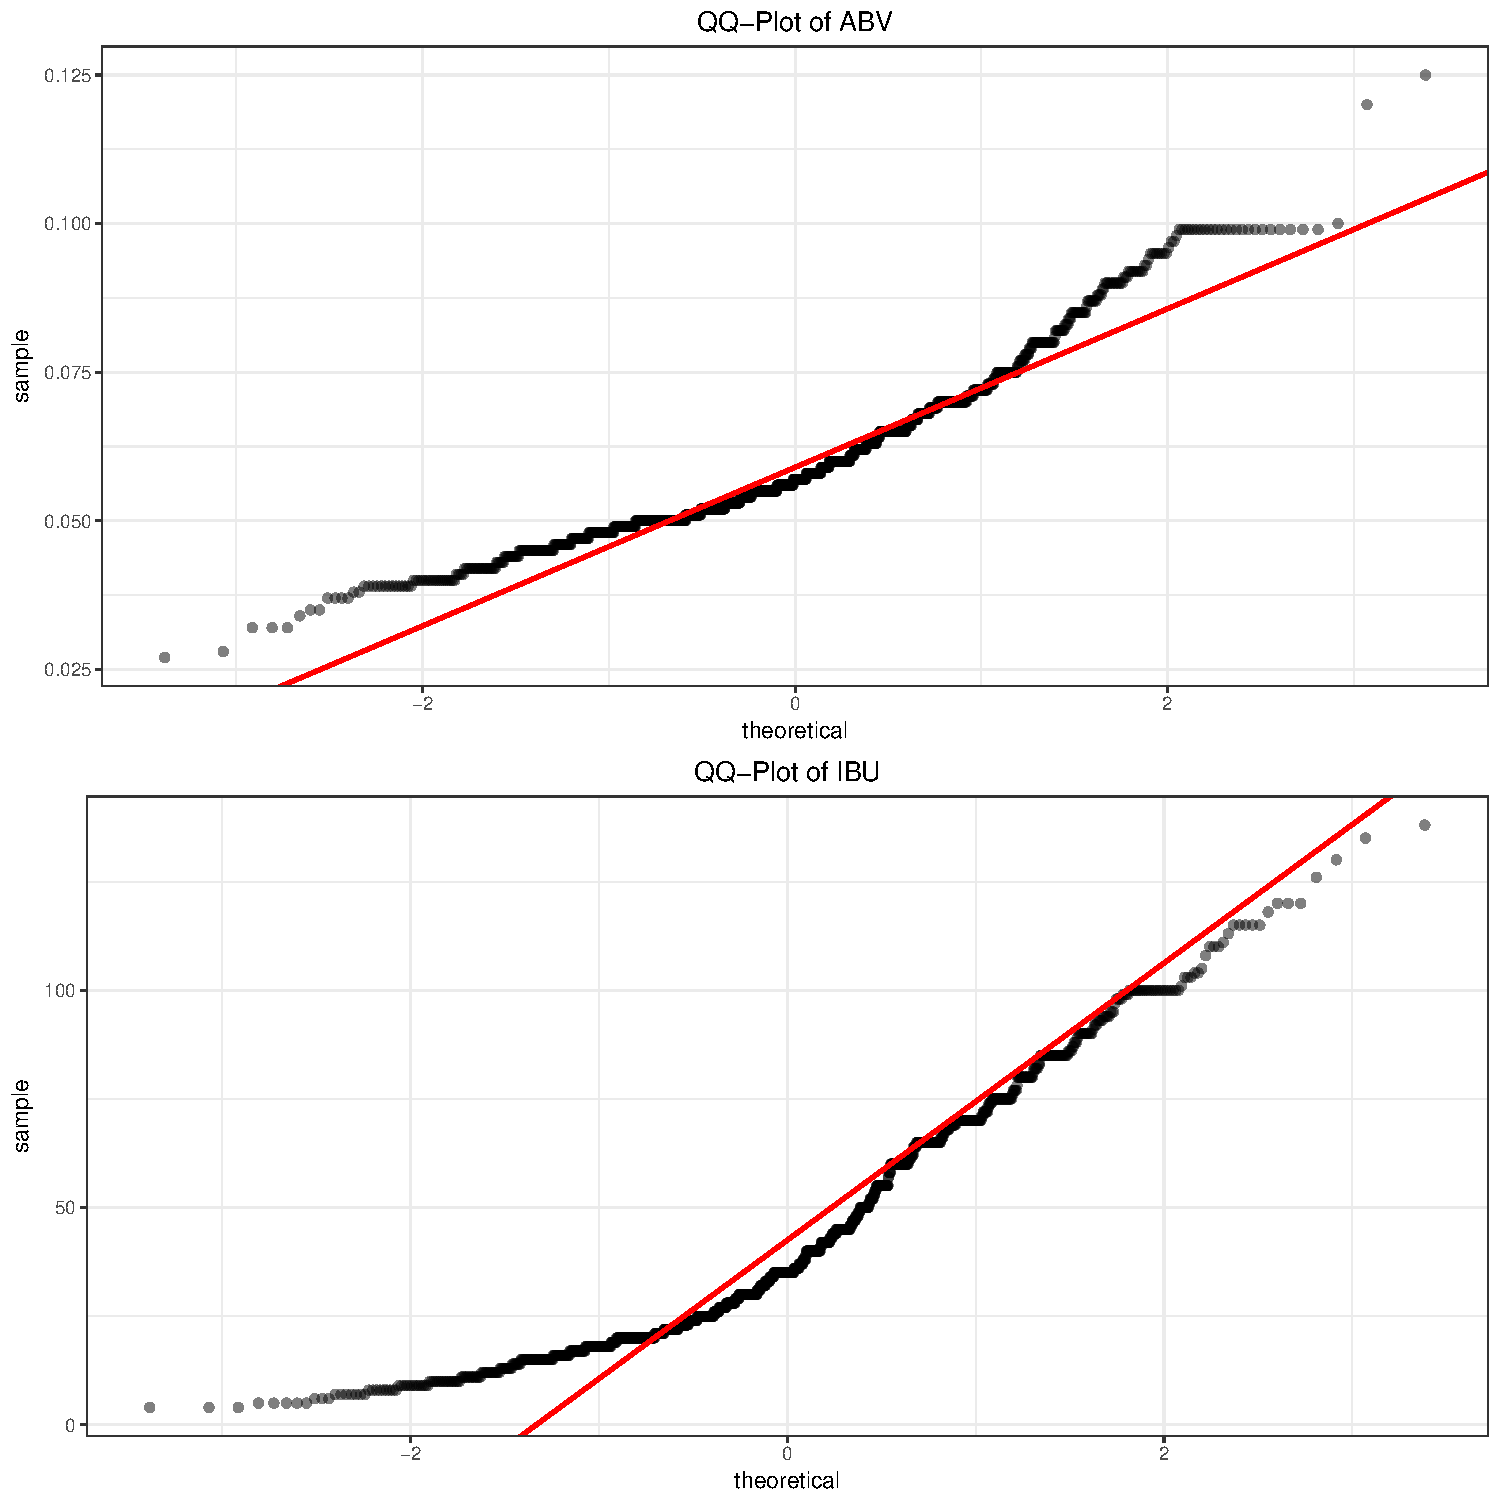
\includegraphics{Analysis_Final_files/figure-latex/unnamed-chunk-24-1} \end{center}

\paragraph{Histogram - Check for
Normality}\label{histogram---check-for-normality}

\begin{Shaded}
\begin{Highlighting}[]
\CommentTok{# Histograms of IBU and ABV}

\NormalTok{hist_ibu <-}\StringTok{ }\KeywordTok{ggplot}\NormalTok{(styles }\OperatorTok\StringTok{ }\KeywordTok{na.omit}\NormalTok{(ibu)) }\OperatorTok{+}
\StringTok{              }\KeywordTok{geom_histogram}\NormalTok{(}\KeywordTok{aes}\NormalTok{(}\DataTypeTok{x=}\NormalTok{ibu)) }\OperatorTok{+}
\StringTok{              }\KeywordTok{theme}\NormalTok{(}\DataTypeTok{text =} \KeywordTok{element_text}\NormalTok{(}\DataTypeTok{size=}\DecValTok{10}\NormalTok{),}
                  \DataTypeTok{axis.text.x =} \KeywordTok{element_text}\NormalTok{(}\DataTypeTok{angle=}\DecValTok{90}\NormalTok{, }\DataTypeTok{hjust=}\DecValTok{1}\NormalTok{)) }

\NormalTok{hist_abv <-}\StringTok{ }\KeywordTok{ggplot}\NormalTok{(styles }\OperatorTok\StringTok{ }\KeywordTok{na.omit}\NormalTok{(abv)) }\OperatorTok{+}
\StringTok{              }\KeywordTok{geom_histogram}\NormalTok{(}\KeywordTok{aes}\NormalTok{(}\DataTypeTok{x=}\NormalTok{abv)) }\OperatorTok{+}
\StringTok{              }\KeywordTok{theme}\NormalTok{(}\DataTypeTok{text =} \KeywordTok{element_text}\NormalTok{(}\DataTypeTok{size=}\DecValTok{10}\NormalTok{),}
                  \DataTypeTok{axis.text.x =} \KeywordTok{element_text}\NormalTok{(}\DataTypeTok{angle=}\DecValTok{90}\NormalTok{, }\DataTypeTok{hjust=}\DecValTok{1}\NormalTok{)) }


\KeywordTok{grid.arrange}\NormalTok{(hist_abv, hist_ibu)}
\end{Highlighting}
\end{Shaded}

\begin{center}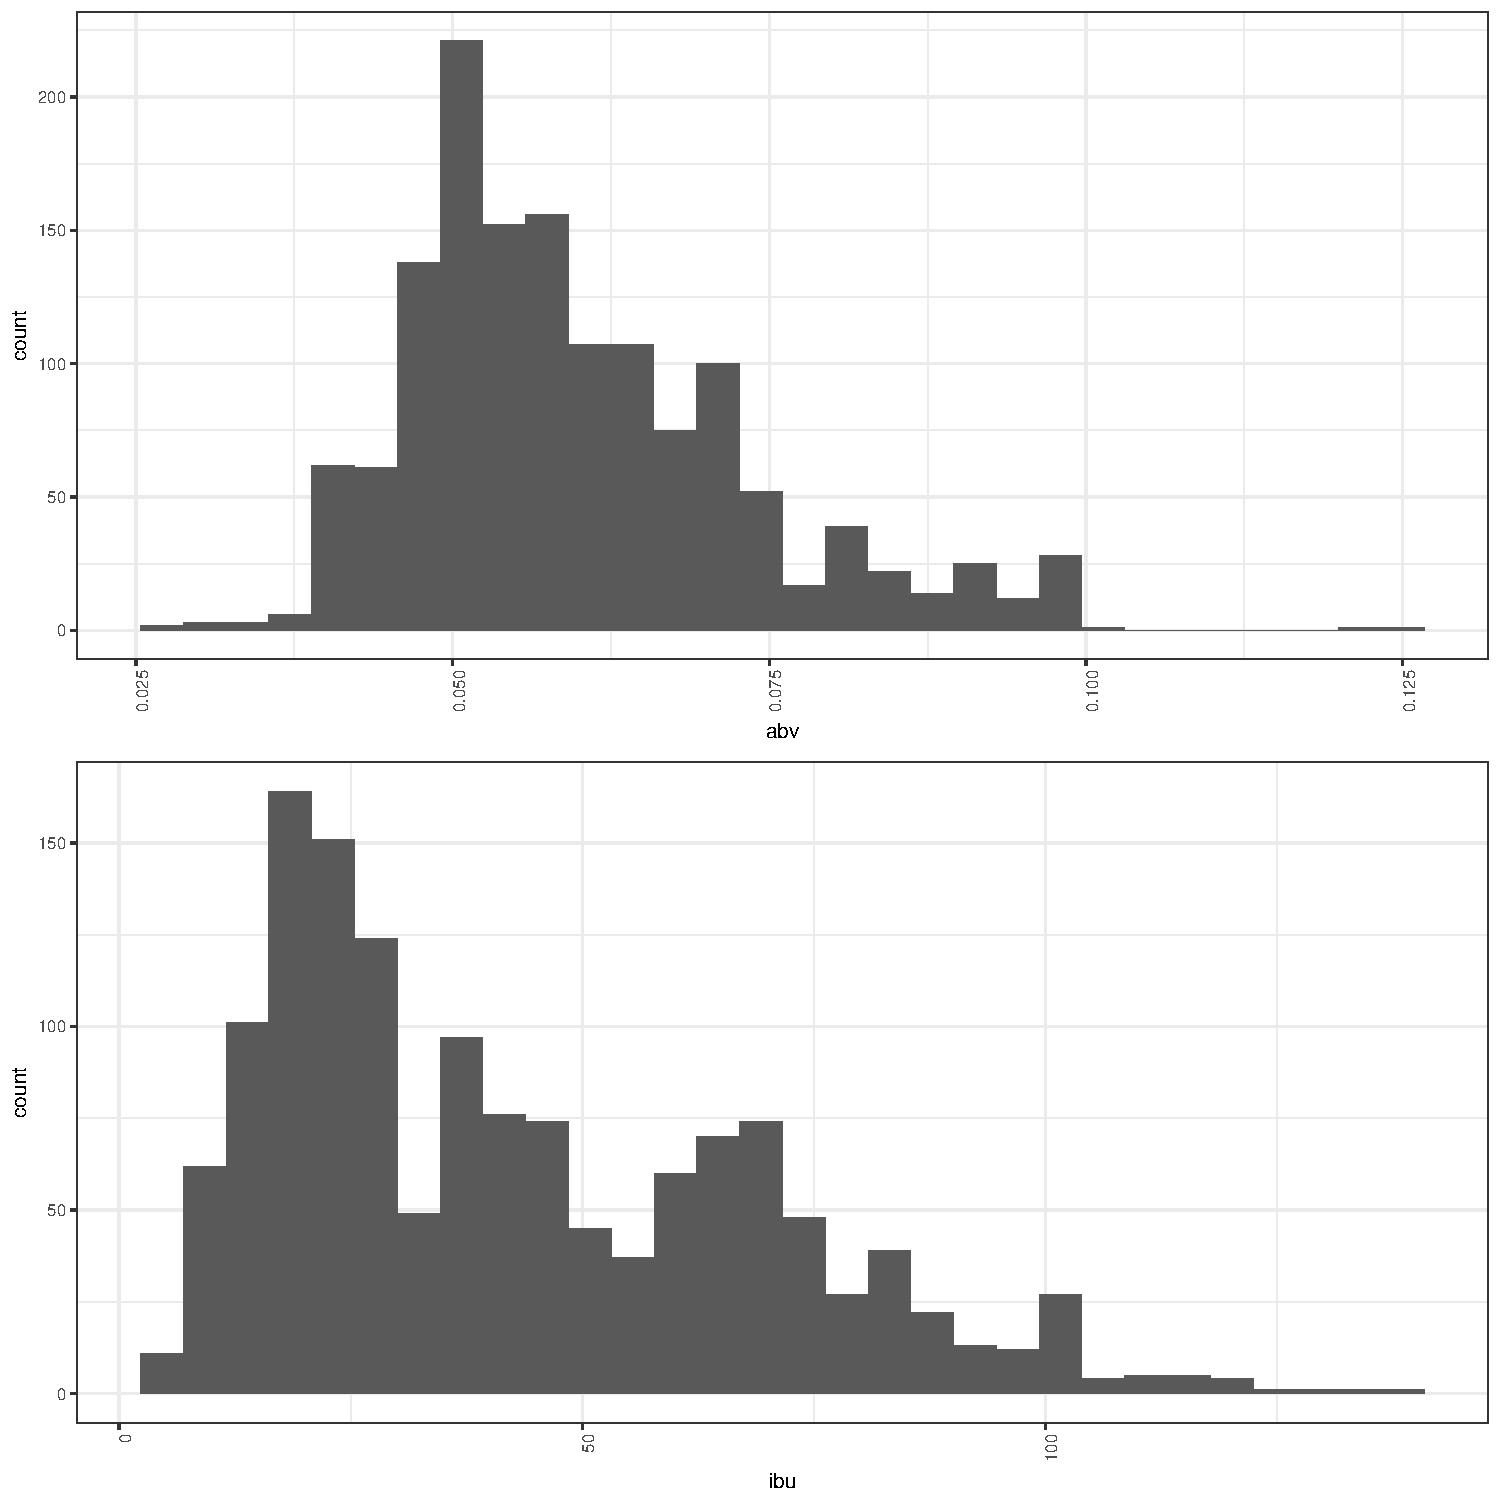
\includegraphics{Analysis_Final_files/figure-latex/unnamed-chunk-25-1} \end{center}

\paragraph{Boxplot - Check for
Outliers}\label{boxplot---check-for-outliers}

\begin{Shaded}
\begin{Highlighting}[]
\CommentTok{# Boxplots of IBU and ABV}


\NormalTok{ibu_outliers <-}\StringTok{ }\KeywordTok{boxplot}\NormalTok{(styles}\OperatorTok{$}\NormalTok{ibu, }\DataTypeTok{plot =} \OtherTok{FALSE}\NormalTok{)[[}\StringTok{"out"}\NormalTok{]]}

\NormalTok{abv_outliers <-}\StringTok{ }\KeywordTok{boxplot}\NormalTok{(styles}\OperatorTok{$}\NormalTok{abv, }\DataTypeTok{plot =} \OtherTok{FALSE}\NormalTok{)[[}\StringTok{"out"}\NormalTok{]]}


\NormalTok{x<-}\KeywordTok{boxplot}\NormalTok{(styles}\OperatorTok{$}\NormalTok{ibu, }\DataTypeTok{plot =} \OtherTok{FALSE}\NormalTok{)}


\NormalTok{bp_abv <-}\StringTok{ }\KeywordTok{ggplot}\NormalTok{((styles }\OperatorTok\StringTok{ }\KeywordTok{drop_na}\NormalTok{(abv)), }\KeywordTok{aes}\NormalTok{(}\DataTypeTok{x=}\StringTok{""}\NormalTok{, }\DataTypeTok{y=}\NormalTok{abv)) }\OperatorTok{+}
\StringTok{      }\KeywordTok{geom_point}\NormalTok{(}\KeywordTok{aes}\NormalTok{(}\DataTypeTok{fill =} \KeywordTok{ifelse}\NormalTok{((abv }\OperatorTok\StringTok{ }\NormalTok{abv_outliers),}\StringTok{"Outlier"}\NormalTok{,}\StringTok{"Valid"}\NormalTok{)), }
                 \DataTypeTok{size =} \DecValTok{4}\NormalTok{, }
                 \DataTypeTok{shape =} \DecValTok{21}\NormalTok{, }
                 \DataTypeTok{position =} \KeywordTok{position_jitter}\NormalTok{())}\OperatorTok{+}
\StringTok{      }\KeywordTok{stat_boxplot}\NormalTok{(}\DataTypeTok{geom =}\StringTok{'errorbar'}\NormalTok{) }\OperatorTok{+}
\StringTok{      }\KeywordTok{geom_boxplot}\NormalTok{(}\DataTypeTok{alpha=}\NormalTok{.}\DecValTok{5}\NormalTok{, }
                   \DataTypeTok{outlier.shape =} \OtherTok{NA}\NormalTok{) }\OperatorTok{+}
\StringTok{      }\KeywordTok{guides}\NormalTok{(}\DataTypeTok{fill=}\KeywordTok{guide_legend}\NormalTok{(}\DataTypeTok{title=} \OtherTok{NULL}\NormalTok{)) }\OperatorTok{+}
\StringTok{      }\KeywordTok{xlab}\NormalTok{(}\OtherTok{NULL}\NormalTok{) }\OperatorTok{+}
\StringTok{      }\KeywordTok{ylab}\NormalTok{(}\StringTok{"Alcohol by Volume (%)"}\NormalTok{) }\OperatorTok{+}
\StringTok{      }\KeywordTok{scale_y_continuous}\NormalTok{(}\DataTypeTok{position =} \StringTok{"right"}\NormalTok{, }
                         \DataTypeTok{breaks =} \KeywordTok{c}\NormalTok{(.}\DecValTok{025}\NormalTok{, .}\DecValTok{05}\NormalTok{, .}\DecValTok{075}\NormalTok{, .}\DecValTok{1}\NormalTok{, .}\DecValTok{125}\NormalTok{), }
                         \DataTypeTok{limits =} \KeywordTok{c}\NormalTok{(}\FloatTok{0.025}\NormalTok{, .}\DecValTok{125}\NormalTok{)) }\OperatorTok{+}
\StringTok{      }\KeywordTok{scale_fill_manual}\NormalTok{(}\DataTypeTok{values =} \KeywordTok{c}\NormalTok{(}\StringTok{'#cc0606'}\NormalTok{, abv_fill)) }\OperatorTok{+}
\StringTok{      }\KeywordTok{theme}\NormalTok{(}\DataTypeTok{plot.title =} \KeywordTok{element_text}\NormalTok{(}\DataTypeTok{hjust =} \FloatTok{0.5}\NormalTok{, }\DataTypeTok{size =} \DecValTok{22}\NormalTok{),}
            \DataTypeTok{axis.title.y=}\KeywordTok{element_blank}\NormalTok{()) }\OperatorTok{+}
\StringTok{      }\KeywordTok{coord_flip}\NormalTok{()}



\NormalTok{bp_ibu <-}\StringTok{ }\KeywordTok{ggplot}\NormalTok{((styles }\OperatorTok\StringTok{ }\KeywordTok{drop_na}\NormalTok{(ibu)), }\KeywordTok{aes}\NormalTok{(}\DataTypeTok{x=}\StringTok{""}\NormalTok{, }\DataTypeTok{y=}\NormalTok{ibu)) }\OperatorTok{+}
\StringTok{      }\KeywordTok{geom_point}\NormalTok{(}\KeywordTok{aes}\NormalTok{(}\DataTypeTok{fill =} \KeywordTok{ifelse}\NormalTok{((ibu }\OperatorTok\StringTok{ }\NormalTok{ibu_outliers),}\StringTok{"Outlier"}\NormalTok{,}\StringTok{"Valid"}\NormalTok{)),}
                 \DataTypeTok{size =} \DecValTok{4}\NormalTok{, }
                 \DataTypeTok{shape =} \DecValTok{21}\NormalTok{, }
                 \DataTypeTok{position =} \KeywordTok{position_jitter}\NormalTok{())}\OperatorTok{+}
\StringTok{      }\KeywordTok{stat_boxplot}\NormalTok{(}\DataTypeTok{geom =}\StringTok{'errorbar'}\NormalTok{) }\OperatorTok{+}
\StringTok{      }\KeywordTok{geom_boxplot}\NormalTok{(}\DataTypeTok{alpha =}\NormalTok{ .}\DecValTok{5}\NormalTok{, }
                   \DataTypeTok{outlier.shape =} \OtherTok{NA}\NormalTok{) }\OperatorTok{+}
\StringTok{      }\KeywordTok{guides}\NormalTok{(}\DataTypeTok{fill=}\KeywordTok{guide_legend}\NormalTok{(}\DataTypeTok{title=} \OtherTok{NULL}\NormalTok{)) }\OperatorTok{+}
\StringTok{      }\KeywordTok{xlab}\NormalTok{(}\OtherTok{NULL}\NormalTok{) }\OperatorTok{+}
\StringTok{      }\KeywordTok{ylab}\NormalTok{(}\StringTok{"International Bitterness Units (IBU)"}\NormalTok{) }\OperatorTok{+}
\StringTok{      }\KeywordTok{scale_y_continuous}\NormalTok{(}\DataTypeTok{breaks =} \KeywordTok{c}\NormalTok{(}\DecValTok{0}\NormalTok{, }\DecValTok{25}\NormalTok{, }\DecValTok{50}\NormalTok{, }\DecValTok{75}\NormalTok{, }\DecValTok{100}\NormalTok{, }\DecValTok{125}\NormalTok{, }\DecValTok{150}\NormalTok{), }
                         \DataTypeTok{limits =} \KeywordTok{c}\NormalTok{(}\DecValTok{0}\NormalTok{, }\DecValTok{150}\NormalTok{)) }\OperatorTok{+}
\StringTok{      }\KeywordTok{scale_fill_manual}\NormalTok{(}\DataTypeTok{values =} \KeywordTok{c}\NormalTok{(}\StringTok{'#cc0606'}\NormalTok{, ibu_fill)) }\OperatorTok{+}
\StringTok{      }\KeywordTok{theme}\NormalTok{(}\DataTypeTok{plot.title =} \KeywordTok{element_text}\NormalTok{(}\DataTypeTok{hjust =} \FloatTok{0.5}\NormalTok{, }\DataTypeTok{size =} \DecValTok{22}\NormalTok{),}
            \DataTypeTok{axis.title.y=}\KeywordTok{element_blank}\NormalTok{()) }\OperatorTok{+}
\StringTok{      }\KeywordTok{coord_flip}\NormalTok{()}

\KeywordTok{grid.arrange}\NormalTok{(bp_abv, bp_ibu)}
\end{Highlighting}
\end{Shaded}

\begin{center}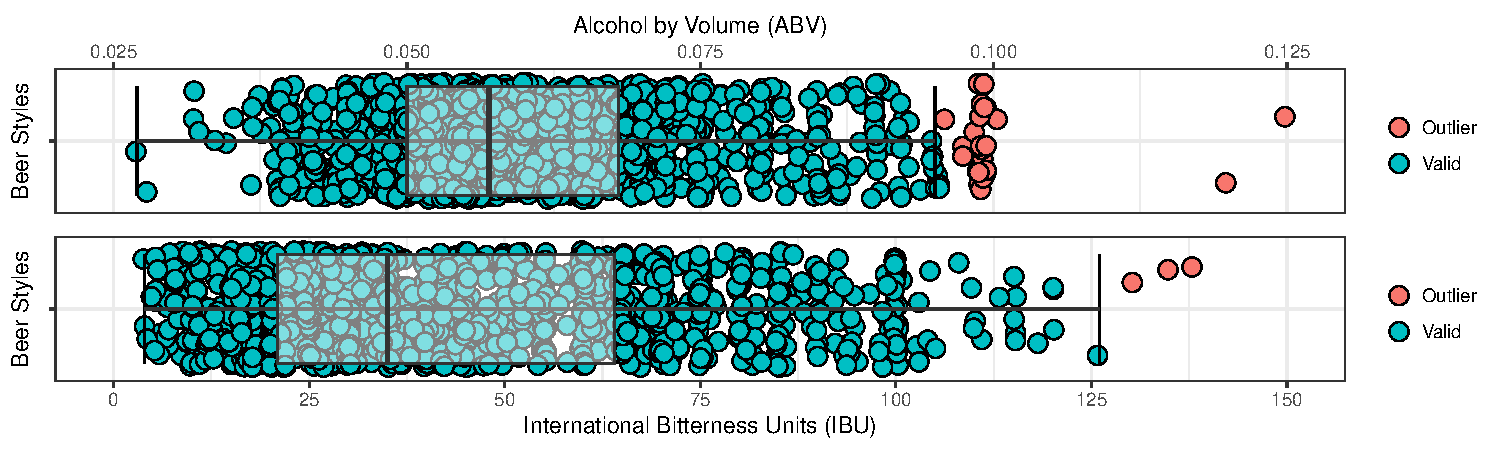
\includegraphics{Analysis_Final_files/figure-latex/unnamed-chunk-26-1} \end{center}

\begin{itemize}
\tightlist
\item
  Due to the lack of normality of the IBU variable and the presence of
  outliers in both variables, we will use the Spearman Rank-Correlation
  test as an alternative to the preferred Pearson Correlation.
\end{itemize}

\paragraph{Significance Testing: Spearman Rank-Order
Correlation}\label{significance-testing-spearman-rank-order-correlation}

\begin{verbatim}
+ More info on Spearman test: https://statistics.laerd.com/statistical-guides/spearmans-rank-order-correlation-statistical-guide.php
\end{verbatim}

\begin{itemize}
\tightlist
\item
  Hypotheses:

  \begin{itemize}
  \tightlist
  \item
    H\textsubscript{o}: \(\rho= 0\)
  \item
    H\textsubscript{A}: \(\rho\neq 0\)
  \end{itemize}
\end{itemize}

\begin{Shaded}
\begin{Highlighting}[]
\NormalTok{alpha <-}\StringTok{ }\FloatTok{0.05}

\CommentTok{# Significance test}
\NormalTok{spear_test_result <-}\StringTok{ }\KeywordTok{cor.test}\NormalTok{(styles}\OperatorTok{$}\NormalTok{ibu, styles}\OperatorTok{$}\NormalTok{abv, }\DataTypeTok{method =} \StringTok{"spearman"}\NormalTok{, }\DataTypeTok{conf.level =}\NormalTok{ alpha, }\DataTypeTok{exact=}\OtherTok{FALSE}\NormalTok{)}

\NormalTok{spear_test_result}
\end{Highlighting}
\end{Shaded}

\begin{verbatim}
## 
##  Spearman's rank correlation rho
## 
## data:  styles$ibu and styles$abv
## S = 153570000, p-value < 2.2e-16
## alternative hypothesis: true rho is not equal to 0
## sample estimates:
##       rho 
## 0.6677798
\end{verbatim}

\begin{Shaded}
\begin{Highlighting}[]
\NormalTok{r_sq <-}\StringTok{ }\NormalTok{spear_test_result[[}\StringTok{"estimate"}\NormalTok{]][[}\StringTok{"rho"}\NormalTok{]]}\OperatorTok{^}\DecValTok{2} \CommentTok{# capture r-squared}

\NormalTok{r_sq}
\end{Highlighting}
\end{Shaded}

\begin{verbatim}
## [1] 0.4459299
\end{verbatim}

\paragraph{Test Conclusion}\label{test-conclusion}

There is strong evidence that the ABV and IBU are positively associated
(p-value \textless{} 0.001 from a Spearman Rank-Order Correlation). At a
95\% confidence level, the IBU rating accounts for 44.59\% of the
variation in the ABV. While IBU and ABV certainly have a correlation,
the correlation is weak (\(r^2 =\) 0.45). Thus, we reject the null
hypothesis that IBU rating and ABV are un-corrolated across the beer
styles in our sample. Beer styles were not randomly assigned to any
treatment and we do not know if the beer data were randomly selected, so
we must limit our results to indicating an association between IBU
rating an ABV. No causality or inferences to larger populations can be
drawn.

\subsection{Conclusion}\label{conclusion}

People all around the world have been drinking beef for centuries. Beer
has been used for refreshment, for refueling, and even for remittance. A
survey of craft brewers in the US shows that beer is still a favorite,
mainstream beverage.

We found that there is at least one craft brewery in every state with an
average brewery to citizen ratio of 1:125,000. There are more than 91
varieties of beer being brewed with a range of strength (alcohol content
and bitterness). The most popular craft beer being brewed is Y with an
ABV of Z and an IBU of AA which puts it at the BB percentile on both
scales.

We determined that there is a distinct positive correlation between
alcohol content and bitterness.

With so many breweries and so many styles of beer, one might expect that
all of the beer bases are covered\ldots{}one would be wrong. There are a
handful of beer types that are statistically under-represented. An
enterprising brewer might want to consider exploiting these overlooked
beers to become a major producer of a niche style.

This investigation focused specifically on ``craft brewers.'' A more
complete investigation could be undertaken to include all commercial
breweries including brew-pub/micro-brewers as well as large, industrial
brewers. Our hypothesis for a more complete investigation would be a
``thickening'' of the middle of the beer type distribution. That is, big
brewers tend to brew the most popular beers whereas craft and
micro-brewers can afford to (or choose to) push the boundaries and
``live in the tails'' of the distribution.

\subsection{Appendex}\label{appendex}

\paragraph{Session Info}\label{session-info}

\begin{Shaded}
\begin{Highlighting}[]
\KeywordTok{sessionInfo}\NormalTok{()}
\end{Highlighting}
\end{Shaded}

R version 3.5.0 (2018-04-23) Platform: x86\_64-w64-mingw32/x64 (64-bit)
Running under: Windows 10 x64 (build 16299)

Matrix products: default

locale: {[}1{]} LC\_COLLATE=English\_United States.1252 {[}2{]}
LC\_CTYPE=English\_United States.1252\\
{[}3{]} LC\_MONETARY=English\_United States.1252 {[}4{]} LC\_NUMERIC=C\\
{[}5{]} LC\_TIME=English\_United States.1252

attached base packages: {[}1{]} stats graphics grDevices utils datasets
methods base

other attached packages: {[}1{]} bindrcpp\_0.2.2 gridExtra\_2.3
magrittr\_1.5\\
{[}4{]} summarytools\_0.8.5 RColorBrewer\_1.1-2 maps\_3.3.0\\
{[}7{]} ggplot2\_2.2.1 knitr\_1.20 tidyr\_0.8.1\\
{[}10{]} dplyr\_0.7.5

loaded via a namespace (and not attached): {[}1{]} Rcpp\_0.12.17
highr\_0.7 pillar\_1.2.3\\
{[}4{]} compiler\_3.5.0 pryr\_0.1.4 plyr\_1.8.4\\
{[}7{]} bindr\_0.1.1 bitops\_1.0-6 tools\_3.5.0\\
{[}10{]} digest\_0.6.15 lubridate\_1.7.4 evaluate\_0.10.1\\
{[}13{]} tibble\_1.4.2 gtable\_0.2.0 pkgconfig\_2.0.1\\
{[}16{]} rlang\_0.2.1 cli\_1.0.0 yaml\_2.1.19\\
{[}19{]} stringr\_1.3.1 rprojroot\_1.3-2 grid\_3.5.0\\
{[}22{]} tidyselect\_0.2.4 glue\_1.2.0 R6\_2.2.2\\
{[}25{]} rmarkdown\_1.10 pander\_0.6.1 purrr\_0.2.5\\
{[}28{]} rapportools\_1.0 backports\_1.1.2 scales\_0.5.0\\
{[}31{]} codetools\_0.2-15 htmltools\_0.3.6 matrixStats\_0.53.1 {[}34{]}
assertthat\_0.2.0 colorspace\_1.3-2 labeling\_0.3\\
{[}37{]} utf8\_1.1.4 stringi\_1.1.7 RCurl\_1.95-4.10\\
{[}40{]} lazyeval\_0.2.1 munsell\_0.5.0 crayon\_1.3.4

\paragraph{Map of Max ABV by State}\label{map-of-max-abv-by-state}

\begin{Shaded}
\begin{Highlighting}[]
\CommentTok{# Map MAX ABV by STATE}

\NormalTok{x <-}\StringTok{ }\KeywordTok{select}\NormalTok{(merged_data, state, abv) }\OperatorTok
\StringTok{                   }\KeywordTok{na.omit}\NormalTok{() }\OperatorTok
\StringTok{                   }\KeywordTok{group_by}\NormalTok{(state) }\OperatorTok
\StringTok{                    }\KeywordTok{summarise_all}\NormalTok{(max) }\OperatorTok
\StringTok{                   }\KeywordTok{arrange}\NormalTok{(}\KeywordTok{desc}\NormalTok{(abv)) }\OperatorTok
\StringTok{                    }\KeywordTok{left_join}\NormalTok{(state_ll, }\DataTypeTok{by=}\KeywordTok{c}\NormalTok{(}\StringTok{"state"}\NormalTok{ =}\StringTok{ "Abbr"}\NormalTok{))}

\NormalTok{breweries_geo2 <-}\StringTok{ }\NormalTok{x }\OperatorTok
\StringTok{                  }\KeywordTok{inner_join}\NormalTok{(states, }\DataTypeTok{by =} \KeywordTok{c}\NormalTok{(}\StringTok{"name"}\NormalTok{ =}\StringTok{ "name"}\NormalTok{)) }





\KeywordTok{ggplot}\NormalTok{((breweries_geo2 }\OperatorTok\StringTok{ }\KeywordTok{arrange}\NormalTok{(}\KeywordTok{desc}\NormalTok{(abv))), }
       \KeywordTok{aes}\NormalTok{(}\DataTypeTok{group =}\NormalTok{ state, }\DataTypeTok{stat=}\StringTok{"identity"}\NormalTok{)) }\OperatorTok{+}
\StringTok{  }\KeywordTok{geom_polygon}\NormalTok{(}\KeywordTok{aes}\NormalTok{(}\DataTypeTok{x =}\NormalTok{ long, }
                   \DataTypeTok{y =}\NormalTok{ lat, }
                   \DataTypeTok{group=}\NormalTok{group, }
                   \DataTypeTok{fill=}\NormalTok{abv), }
               \DataTypeTok{color =} \StringTok{"black"}\NormalTok{) }\OperatorTok{+}\StringTok{ }
\StringTok{  }\KeywordTok{geom_text}\NormalTok{(}\DataTypeTok{data =}\NormalTok{ (x }\OperatorTok\StringTok{ }
\StringTok{                    }\KeywordTok{filter}\NormalTok{(}\OperatorTok{!}\NormalTok{(state }\OperatorTok\StringTok{ }\KeywordTok{c}\NormalTok{(}\StringTok{"AK"}\NormalTok{, }\StringTok{"DC"}\NormalTok{, }\StringTok{"HI"}\NormalTok{)))), }\CommentTok{#filter to continental 50 states}
            \KeywordTok{aes}\NormalTok{(}\DataTypeTok{x =}\NormalTok{ lon_center, }
                \DataTypeTok{y =}\NormalTok{ lat_center, }
                \DataTypeTok{label =} \KeywordTok{as.character}\NormalTok{(}\KeywordTok{round}\NormalTok{(abv, }\DecValTok{2}\NormalTok{))),}
            \DataTypeTok{color =} \StringTok{'white'}\NormalTok{,}
            \DataTypeTok{size =} \DecValTok{4}
\NormalTok{            ) }\OperatorTok{+}
\StringTok{  }\KeywordTok{scale_fill_gradient}\NormalTok{(}\DataTypeTok{low=}\NormalTok{abv_fill, }\DataTypeTok{high=}\StringTok{'#8E5C05'}\NormalTok{) }\OperatorTok{+}
\StringTok{  }\KeywordTok{guides}\NormalTok{(}\DataTypeTok{fill=}\KeywordTok{guide_legend}\NormalTok{(}\DataTypeTok{title=} \StringTok{"Max ABV"}\NormalTok{)) }\OperatorTok{+}
\StringTok{  }\KeywordTok{coord_fixed}\NormalTok{(}\FloatTok{1.3}\NormalTok{) }\OperatorTok{+}\StringTok{ }\CommentTok{# fix lat/long display ratio}
\StringTok{  }\KeywordTok{ggtitle}\NormalTok{(}\StringTok{"Max ABV by State"}\NormalTok{) }\OperatorTok{+}\StringTok{ }\CommentTok{# set plot title}
\StringTok{  }\KeywordTok{theme}\NormalTok{(}\DataTypeTok{plot.title =} \KeywordTok{element_text}\NormalTok{(}\DataTypeTok{hjust =} \FloatTok{0.5}\NormalTok{)) }\OperatorTok{+}\StringTok{ }\CommentTok{# center plot title}
\StringTok{  }\KeywordTok{theme}\NormalTok{(}\DataTypeTok{legend.position =} \StringTok{"left"}\NormalTok{,}
        \DataTypeTok{axis.title.x=}\KeywordTok{element_blank}\NormalTok{(), }\CommentTok{# hide x axis title}
        \DataTypeTok{axis.text.x=}\KeywordTok{element_blank}\NormalTok{(),  }\CommentTok{# hide x axis text}
        \DataTypeTok{axis.ticks.x=}\KeywordTok{element_blank}\NormalTok{(), }\CommentTok{# hide x axis ticks}
        \DataTypeTok{axis.title.y=}\KeywordTok{element_blank}\NormalTok{(), }\CommentTok{# hide y axis title}
        \DataTypeTok{axis.text.y=}\KeywordTok{element_blank}\NormalTok{(),  }\CommentTok{# hide y axis text}
        \DataTypeTok{axis.ticks.y=}\KeywordTok{element_blank}\NormalTok{()) }\CommentTok{# hide y axis ticks}
\end{Highlighting}
\end{Shaded}

\begin{center}\includegraphics{Analysis_Final_files/figure-latex/unnamed-chunk-29-1} \end{center}

\paragraph{Map of Max IBU by State}\label{map-of-max-ibu-by-state}

\begin{Shaded}
\begin{Highlighting}[]
\CommentTok{# MAX IBU by STATE}

\NormalTok{x <-}\StringTok{ }\KeywordTok{select}\NormalTok{(merged_data, state, ibu) }\OperatorTok
\StringTok{                   }\KeywordTok{na.omit}\NormalTok{() }\OperatorTok
\StringTok{                   }\KeywordTok{group_by}\NormalTok{(state) }\OperatorTok
\StringTok{                    }\KeywordTok{summarise_all}\NormalTok{(max) }\OperatorTok
\StringTok{                   }\KeywordTok{arrange}\NormalTok{(}\KeywordTok{desc}\NormalTok{(ibu)) }\OperatorTok
\StringTok{                    }\KeywordTok{full_join}\NormalTok{(state_ll, }\DataTypeTok{by=}\KeywordTok{c}\NormalTok{(}\StringTok{"state"}\NormalTok{ =}\StringTok{ "Abbr"}\NormalTok{))}

\NormalTok{breweries_geo2 <-}\StringTok{ }\NormalTok{x }\OperatorTok
\StringTok{                  }\KeywordTok{inner_join}\NormalTok{(states, }\DataTypeTok{by =} \KeywordTok{c}\NormalTok{(}\StringTok{"name"}\NormalTok{ =}\StringTok{ "name"}\NormalTok{)) }





\KeywordTok{ggplot}\NormalTok{((breweries_geo2 }\OperatorTok\StringTok{ }\KeywordTok{arrange}\NormalTok{(}\KeywordTok{desc}\NormalTok{(ibu))), }
       \KeywordTok{aes}\NormalTok{(}\DataTypeTok{group =}\NormalTok{ state, }\DataTypeTok{stat=}\StringTok{"identity"}\NormalTok{)) }\OperatorTok{+}
\StringTok{  }\KeywordTok{geom_polygon}\NormalTok{(}\KeywordTok{aes}\NormalTok{(}\DataTypeTok{x =}\NormalTok{ long, }
                   \DataTypeTok{y =}\NormalTok{ lat, }
                   \DataTypeTok{group=}\NormalTok{group, }
                   \DataTypeTok{fill=}\NormalTok{ibu), }
               \DataTypeTok{color =} \StringTok{"black"}\NormalTok{) }\OperatorTok{+}\StringTok{ }
\StringTok{  }\KeywordTok{geom_text}\NormalTok{(}\DataTypeTok{data =}\NormalTok{ (x }\OperatorTok\StringTok{ }
\StringTok{                    }\KeywordTok{filter}\NormalTok{(}\OperatorTok{!}\NormalTok{(state }\OperatorTok\StringTok{ }\KeywordTok{c}\NormalTok{(}\StringTok{"AK"}\NormalTok{, }\StringTok{"DC"}\NormalTok{, }\StringTok{"HI"}\NormalTok{)))), }\CommentTok{#filter to continental 50 states}
            \KeywordTok{aes}\NormalTok{(}\DataTypeTok{x =}\NormalTok{ lon_center, }
                \DataTypeTok{y =}\NormalTok{ lat_center, }
                \DataTypeTok{label =} \KeywordTok{as.character}\NormalTok{(ibu)),}
            \DataTypeTok{color =} \StringTok{'white'}
\NormalTok{            ) }\OperatorTok{+}
\StringTok{  }\KeywordTok{scale_fill_gradient}\NormalTok{(}\DataTypeTok{low=}\NormalTok{ibu_fill, }\DataTypeTok{high=}\StringTok{'#035C64'}\NormalTok{) }\OperatorTok{+}
\StringTok{  }\KeywordTok{guides}\NormalTok{(}\DataTypeTok{fill=}\KeywordTok{guide_legend}\NormalTok{(}\DataTypeTok{title=} \StringTok{"Max IBU"}\NormalTok{)) }\OperatorTok{+}
\StringTok{  }\KeywordTok{coord_fixed}\NormalTok{(}\FloatTok{1.3}\NormalTok{) }\OperatorTok{+}\StringTok{ }\CommentTok{# fix lat/long display ratio}
\StringTok{  }\KeywordTok{ggtitle}\NormalTok{(}\StringTok{"Max IBU by State"}\NormalTok{) }\OperatorTok{+}\StringTok{ }\CommentTok{# set plot title}
\StringTok{  }\KeywordTok{theme}\NormalTok{(}\DataTypeTok{plot.title =} \KeywordTok{element_text}\NormalTok{(}\DataTypeTok{hjust =} \FloatTok{0.5}\NormalTok{)) }\OperatorTok{+}\StringTok{ }\CommentTok{# center plot title}
\StringTok{  }\KeywordTok{theme}\NormalTok{(}\DataTypeTok{legend.position =} \StringTok{"left"}\NormalTok{,}
        \DataTypeTok{axis.title.x=}\KeywordTok{element_blank}\NormalTok{(), }\CommentTok{# hide x axis title}
        \DataTypeTok{axis.text.x=}\KeywordTok{element_blank}\NormalTok{(),  }\CommentTok{# hide x axis text}
        \DataTypeTok{axis.ticks.x=}\KeywordTok{element_blank}\NormalTok{(), }\CommentTok{# hide x axis ticks}
        \DataTypeTok{axis.title.y=}\KeywordTok{element_blank}\NormalTok{(), }\CommentTok{# hide y axis title}
        \DataTypeTok{axis.text.y=}\KeywordTok{element_blank}\NormalTok{(),  }\CommentTok{# hide y axis text}
        \DataTypeTok{axis.ticks.y=}\KeywordTok{element_blank}\NormalTok{()) }\CommentTok{# hide y axis ticks}
\end{Highlighting}
\end{Shaded}

\begin{center}\includegraphics{Analysis_Final_files/figure-latex/unnamed-chunk-30-1} \end{center}


\end{document}
